%! TEX program = pdflatex
%! TEX root = main.tex

\chapter{\texorpdfstring{\MakeUppercase{NCTM Case Study}}{NCTM Case Study}}
\label{sec:nctm}

The National Center for Therapeutics Manufacturing (NCTM)
building was used as a test bed for the methodology. NCTM is a building
located on the campus of Texas A\&M University, in College Station,
Texas. \figref{} \ref{fig:ImageOfNCTMBuilding} shows an image of the
main entrance to the building.

The National Center for Therapeutics Manufacturing (NCTM) combines the
educational and manufacturing focuses of the biopharmaceutical industry.  The
NCTM building is approximately \SI{150000}{\feet\squared} with nearly
\SI{50000}{\feet\squared} of educational facilities that include wet labs,
culture facilities, large lecture halls, and a mock current Good Manufacturing
Practice (cGMP) training suite. Around \SI{120000}{\feet\squared} are on the
first level and \SI{30000}{\feet\squared} are on the second level. 

The cGMP Suite contains modern biopharmaceutical manufacturing equipment
that students can use to learn industry practices. The wet labs are
equipped with chemical fume hoods and the necessary electronic equipment
for following standard operating procedures used in the
biopharmaceutical industry. The two lecture halls seat up to 120 students
and have large floor to ceiling windows. There is also an Apple Computer
laboratory with 48 workstations on the second floor. 

On the academic side, three dedicated outdoor air handling
units (OAHU) serve seven air handling units. Two of the air handling
units are constant speed, and the others are variable air volume. OAHU
1-1 serves its own wet lab and also feeds into AHU 1-1 and AHU 1-2. OAHU
1-2 serves AHU 1-3 and 1-4 on the first floor. OAHU 2-1 serves three
air handlers on the second floor, AHU 2-1, 2-2, and 2-3. 

Various specifications for the air handling units are shown in Tables
\ref{tab:OnOffSched} through \ref{tab:FanSched}.

This document focuses on the academic side of the building since
Utilities and Energy services with Texas A\&M University are only
allowed to make changes to the HVAC system and collect data on this
side. In summary, the relevant facts concerning NCTM are that it houses
several biopharmaceutical labs, it has an academic side that had
available data, and relies on dedicated outdoor air handling units to
pretreat outdoor air. 


\begin{figure}
\centering
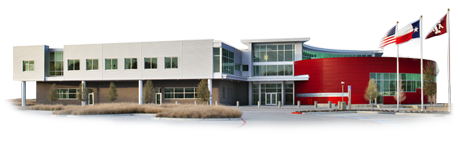
\includegraphics[width=0.9\textwidth]{Images/nctm-building.png}
\caption{Main entrance to the NCTM building at Texas A\&M (\url{https://engineering.tamu.edu/media/15458/nctm-building.png}).}
\label{fig:ImageOfNCTMBuilding}
\end{figure}


\begin{table}
\centering
\caption{Occupied/Unoccupied scheduling for the AHUs as described. }
\label{tab:OnOffSched}
\begin{tabular}{l c c c}
\toprule
Level          & OAHU     & AHU \#  & AHU Schedule    \\
\midrule
Floor 1 Area B & OAHU 1-1 & N/A     & 24/7            \\
Floor 1 Area B & OAHU 1-1 & AHU 1-1 & 24/7            \\
Floor 1 Area B & OAHU 1-1 & AHU 1-2 & 6am - 6pm, M-F  \\
Floor 1 Area A & OAHU 1-2 & AHU 1-3 & 6am - 8pm, M-F  \\
Floor 1 Area A & OAHU 1-2 & AHU 1-4 & 6am - 8pm, M-F  \\
Floor 2        & OAHU 2-1 & AHU 2-1 & 6am - 10pm, M-F \\
Floor 2        & OAHU 2-1 & AHU 2-2 & 6am - 10pm, M-F \\
Floor 2        & OAHU 2-1 & AHU 2-3 & 6am - 10pm, M-F \\
\bottomrule
\end{tabular}
\end{table}


\begin{table}
\caption{Fan schedule information for the dedicated outdoor air handlers.}
\label{tab:OAFanSched}
\centering
\begin{tabular}{l S S}
\toprule
OAHU & {Design OA CFM} & {HP} \\
\midrule
OAHU 1-1 & 12800 & 20 \\
OAHU 1-2 & 4500  & 5  \\
OAHU 2-1 & 2200  & 2  \\
\bottomrule
\multicolumn{1}{r}{Total:} & 19500 & 27 \\
\end{tabular}
\end{table}

\begin{table}
\centering
\caption{Fan schedule information for the AHUs.}
\label{tab:FanSched}
\begin{tabular}{l c S S c}
\toprule
AHU 	& Type	 	& { Total Airflow (CFM) } 	& {HP} 	& OA Served By\\
\midrule
AHU 1-1 & Constant & 3000 & 5   & OAHU 1-1 \\
AHU 1-2 & VAV      & 4800 & 5   & OAHU 1-1 \\
AHU 1-3 & VAV      & 7500 & 7.5 & OAHU 1-2 \\
AHU 1-4 & Constant & 5000 & 7.5 & OAHU 1-2 \\
AHU 2-1 & VAV      & 6000 & 7.5 & OAHU 2-1 \\
AHU 2-2 & VAV      & 8500 & 10  & OAHU 2-1 \\
AHU 2-3 & VAV      & 6000 & 7.5 & OAHU 2-1 \\
\bottomrule
\multicolumn{2}{r}{Total:} & 40800 & 50 &  \\
\end{tabular}
\end{table}

\figref{} \ref{fig:FirstFloorPlanAreaA} through \figref{}
\ref{fig:SecondFloorPlan} show the respective areas that the air
handling units serve. 

\section{Terminal Unit Information}

On the academic side, there are a total of 10 series fan powered terminal units
on the first floor and 18 on the second floor.  \tableref{}
\ref{tab:TerminalUnitInformation} shows the design flowrates and type of space
served for each of the terminal units. 


\begin{table}
\centering
\footnotesize
\caption{Terminal unit information.}
\label{tab:TerminalUnitInformation}
\begin{tabular}{@{}llrl@{}}
\toprule
AHU &  Terminal Unit & \parbox{1.5cm}{\centering Flow\\(CFM) }& Space Served \\ \midrule
%%\parbox{2cm}{AHU-1-1 \\ (5 hp)} & \multicolumn{3}{l}{No boxes - Serves Teaching Module alone, Constant Fan} \\ \midrule
AHU-1-2  & FPVAV-1-7  & 1,400 & Difficult to tell                   \\ \cmidrule(r){2-4}
(5 hp)   & FPVAV-1-8  & 700   & Vestibule/Men's \&  Women's bathroom \\ \cmidrule(r){2-4}
         & FPVAV-1-9  & 1,200 & Stairs/Front Corridor               \\ \cmidrule(r){2-4}
         & FPVAV-1-10 & 1,600 & Hallway                             \\ \midrule
AHU-1-3  & FPVAV-1-1  & 1,480 & Large Auditorium Lecture Hall       \\ \cmidrule(r){2-4}
(7.5 hp) & FPVAV-1-2  & 1,160 & Large Auditorium Lecture Hall       \\ \cmidrule(r){2-4}
         & FPVAV-1-3  & 1,300 & Large Auditorium Lecture Hall       \\ \cmidrule(r){2-4}
         & FPVAV-1-4  & 1,400 & Large Auditorium Lecture Hall       \\ \cmidrule(r){2-4}
         & FPVAV-1-5  & 1,040 & Large Auditorium Lecture Hall       \\ \cmidrule(r){2-4}
         & FPVAV-1-6  & 1,120 & Large Auditorium Lecture Hall       \\ \midrule
%%\parbox{2cm}{AHU-1-4 \\ (7.5 hp)} & \multicolumn{3}{l}{No boxes - Serves open atrium outside lecture halls, constant fan}  \\\midrule
AHU-2-1  & FPVAV-2-1  & 2,000 & Large Study Area                                                         \\ \cmidrule(r){2-4}
(7.5 hp) & FPVAV-2-2  & 2,200 & Large Study Area                                                         \\ \cmidrule(r){2-4}
         & FPVAV-2-3  & 1,800 & Open Corridor                                                            \\ \midrule
AHU-2-2  & FPVAV-2-9  & 2,400 & Computer Lab                                                             \\ \cmidrule(r){2-4}
(10 hp)  & FPVAV-2-12 & 500   & Kitchen/Mail Room                                                        \\ \cmidrule(r){2-4}
         & FPVAV-2-13 & 1,000 & Open Corridor                                                            \\ \cmidrule(r){2-4}
         & FPVAV-2-14 & 850   & \pbox{\textwidth}{Men's/Women's Restroom \\ Copy/Mail  \\ Waiting Area } \\ \cmidrule(r){2-4}
         & FPVAV-2-15 & 1,400 & Reception/Seating/Admin Lobby                                            \\ \cmidrule(r){2-4}
         & FPVAV-2-16 & 500   & Small Conference Room                                                    \\ \cmidrule(r){2-4}
         & FPVAV-2-17 & 1,280 & 4 Small Offices                                                          \\ \cmidrule(r){2-4}
         & FPVAV-2-18 & 600   & Large Office                                                             \\ \midrule
AHU-2-3  & FPVAV-2-4  & 2,000 & Open Corridor                                                            \\ \cmidrule(r){2-4}
(7.5 hp) & FPVAV-2-5  & 600   & Open Seating                                                             \\ \cmidrule(r){2-4}
         & FPVAV-2-6  & 400   & Small Conference Room                                                    \\ \cmidrule(r){2-4}
         & FPVAV-2-7  & 200   & Office                                                                   \\ \cmidrule(r){2-4}
         & FPVAV-2-8  & 1,200 & Visitor Conference                                                       \\ \cmidrule(r){2-4}
         & FPVAV-2-10 & 540   & 3 Sponsor Offices                                                        \\ \cmidrule(r){2-4}
         & FPVAV-2-11 & 560   & 3 Sponsor Offices                                                        \\ \bottomrule
\end{tabular}
\end{table}

\begin{figure}
    \centering
    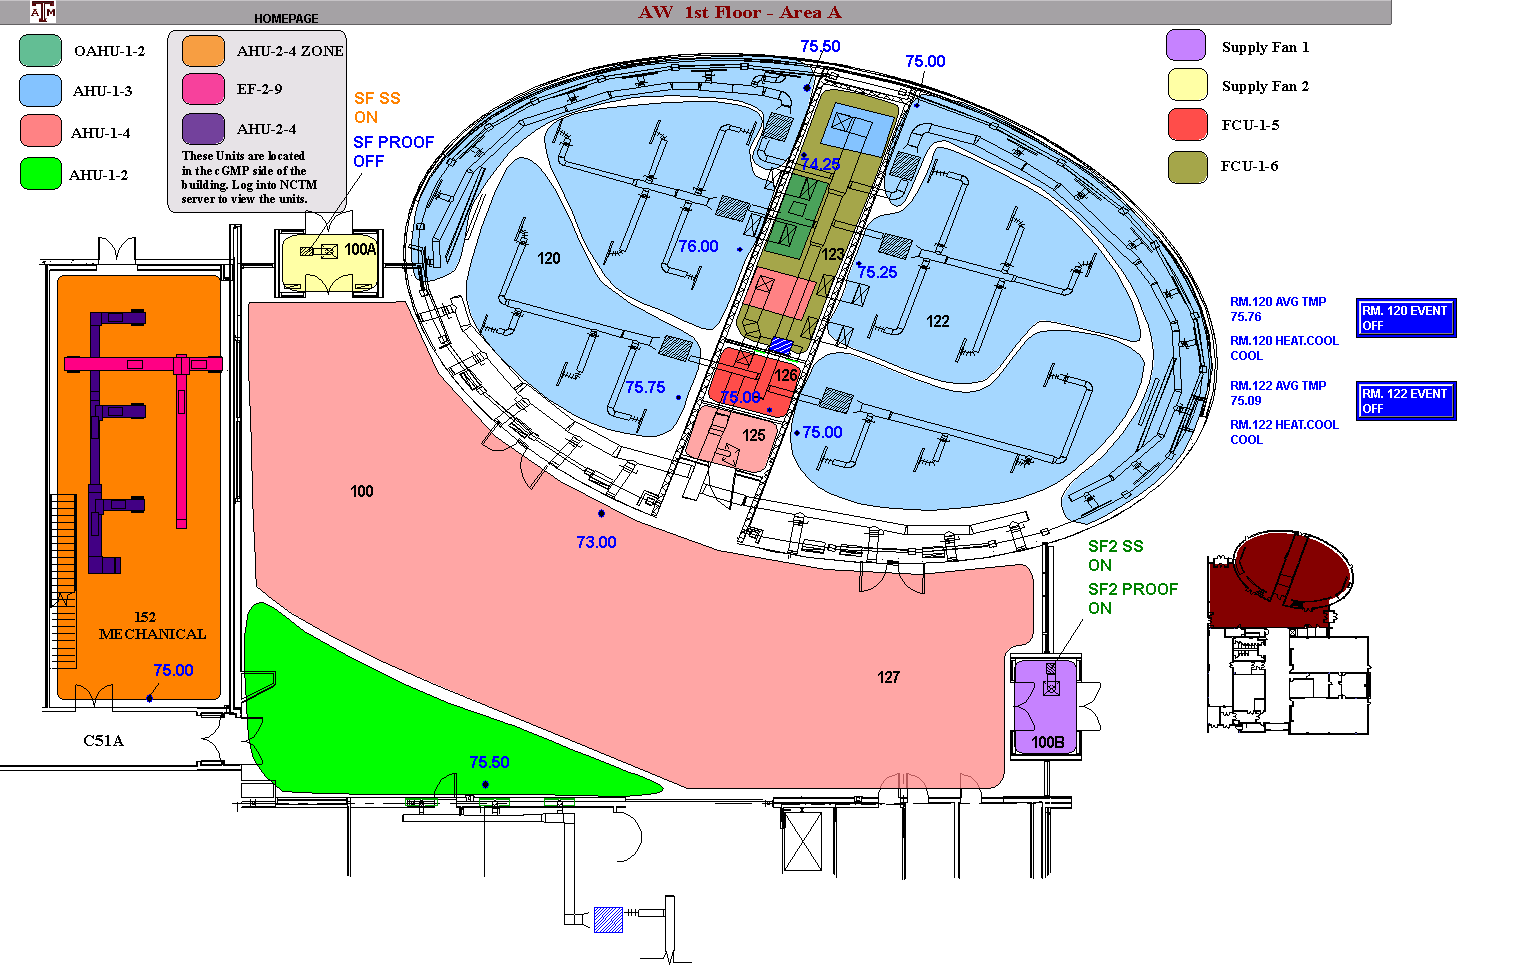
\includegraphics[width=\textwidth]{Images/FirstFloorPlanAreaA.PNG}
    \caption{First floor plan for Area A.}
    \label{fig:FirstFloorPlanAreaA}
\end{figure}

%\begin{landscape}
    %\begin{figure}
        %\centering
        %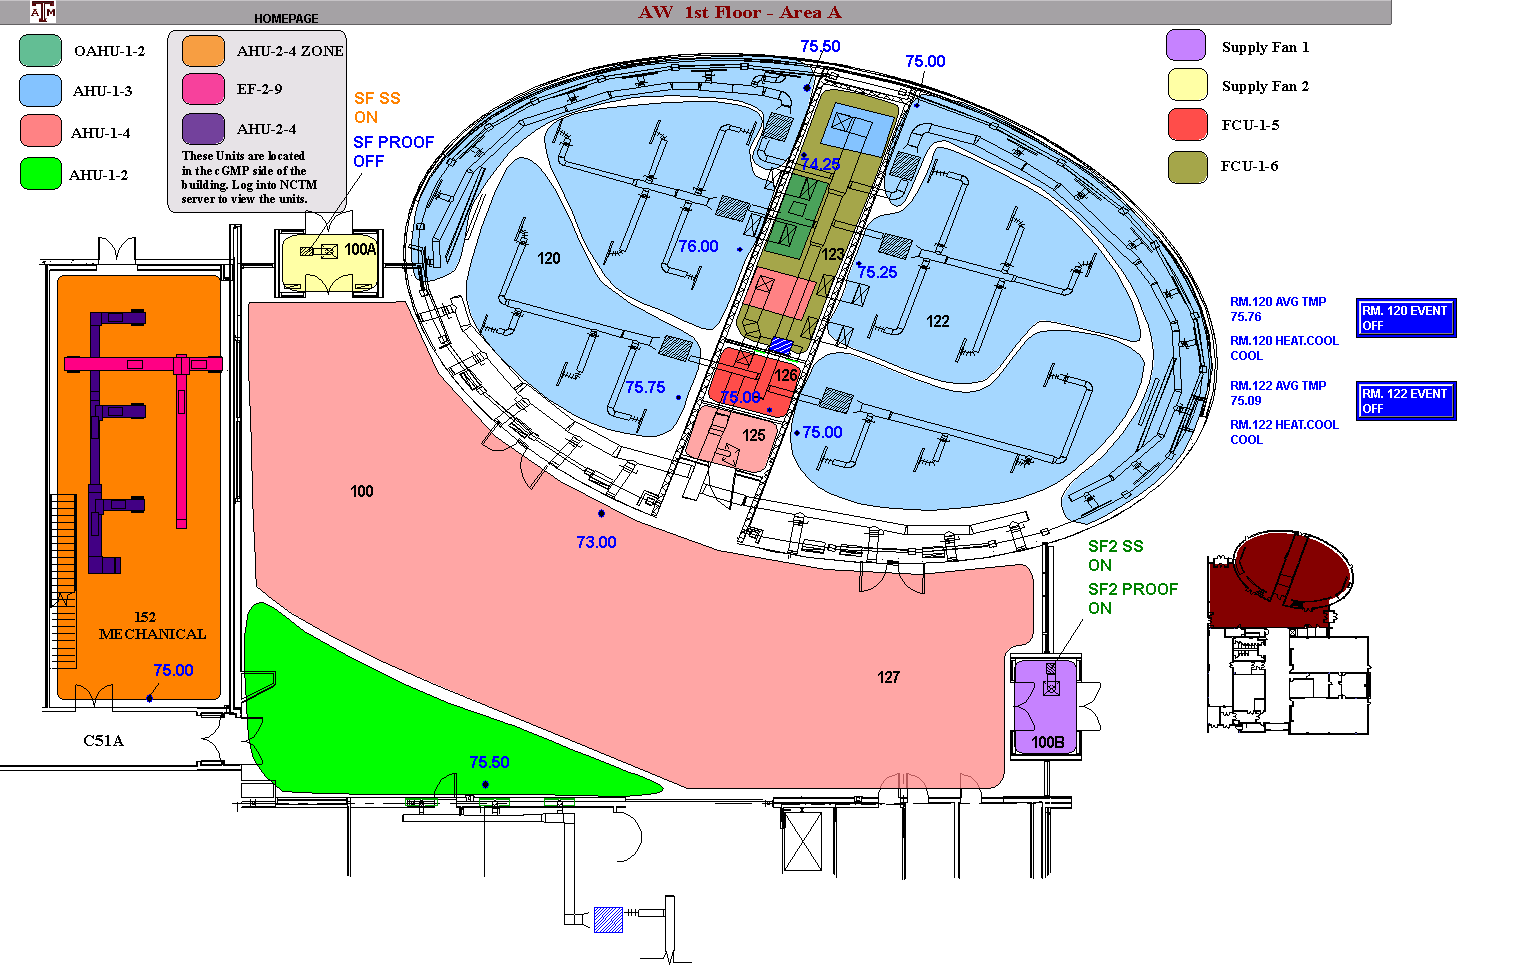
\includegraphics[height=\textwidth]{Images/FirstFloorPlanAreaA.PNG}
        %\caption{First floor plan for Area A.}
        %\label{fig:FirstFloorPlanAreaA}
    %\end{figure}
%\end{landscape}

\begin{figure}
    \centering
    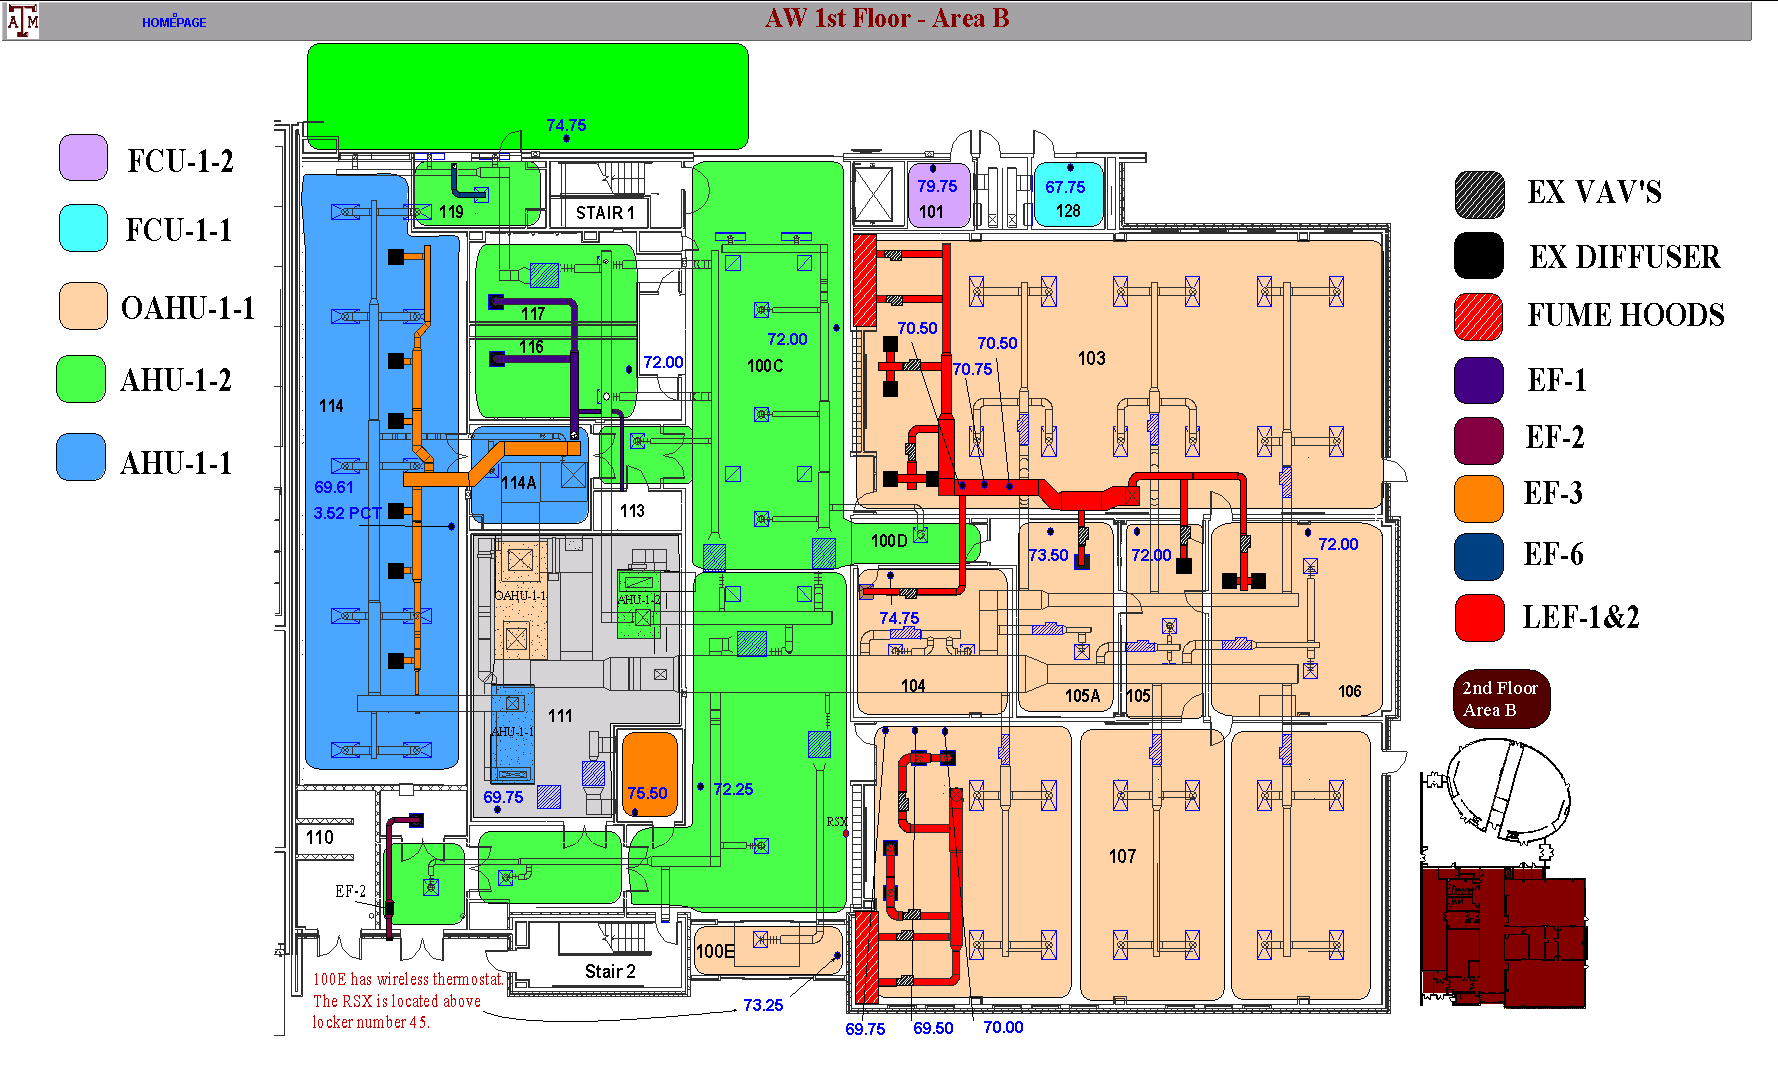
\includegraphics[width=\textwidth]{Images/FirstFloorPlanAreaB.PNG}
    \caption{First floor plan for Area B.}
    \label{fig:FirstFloorPlanAreaB}
\end{figure}

%\begin{landscape}
    %\begin{figure}
        %\centering
        %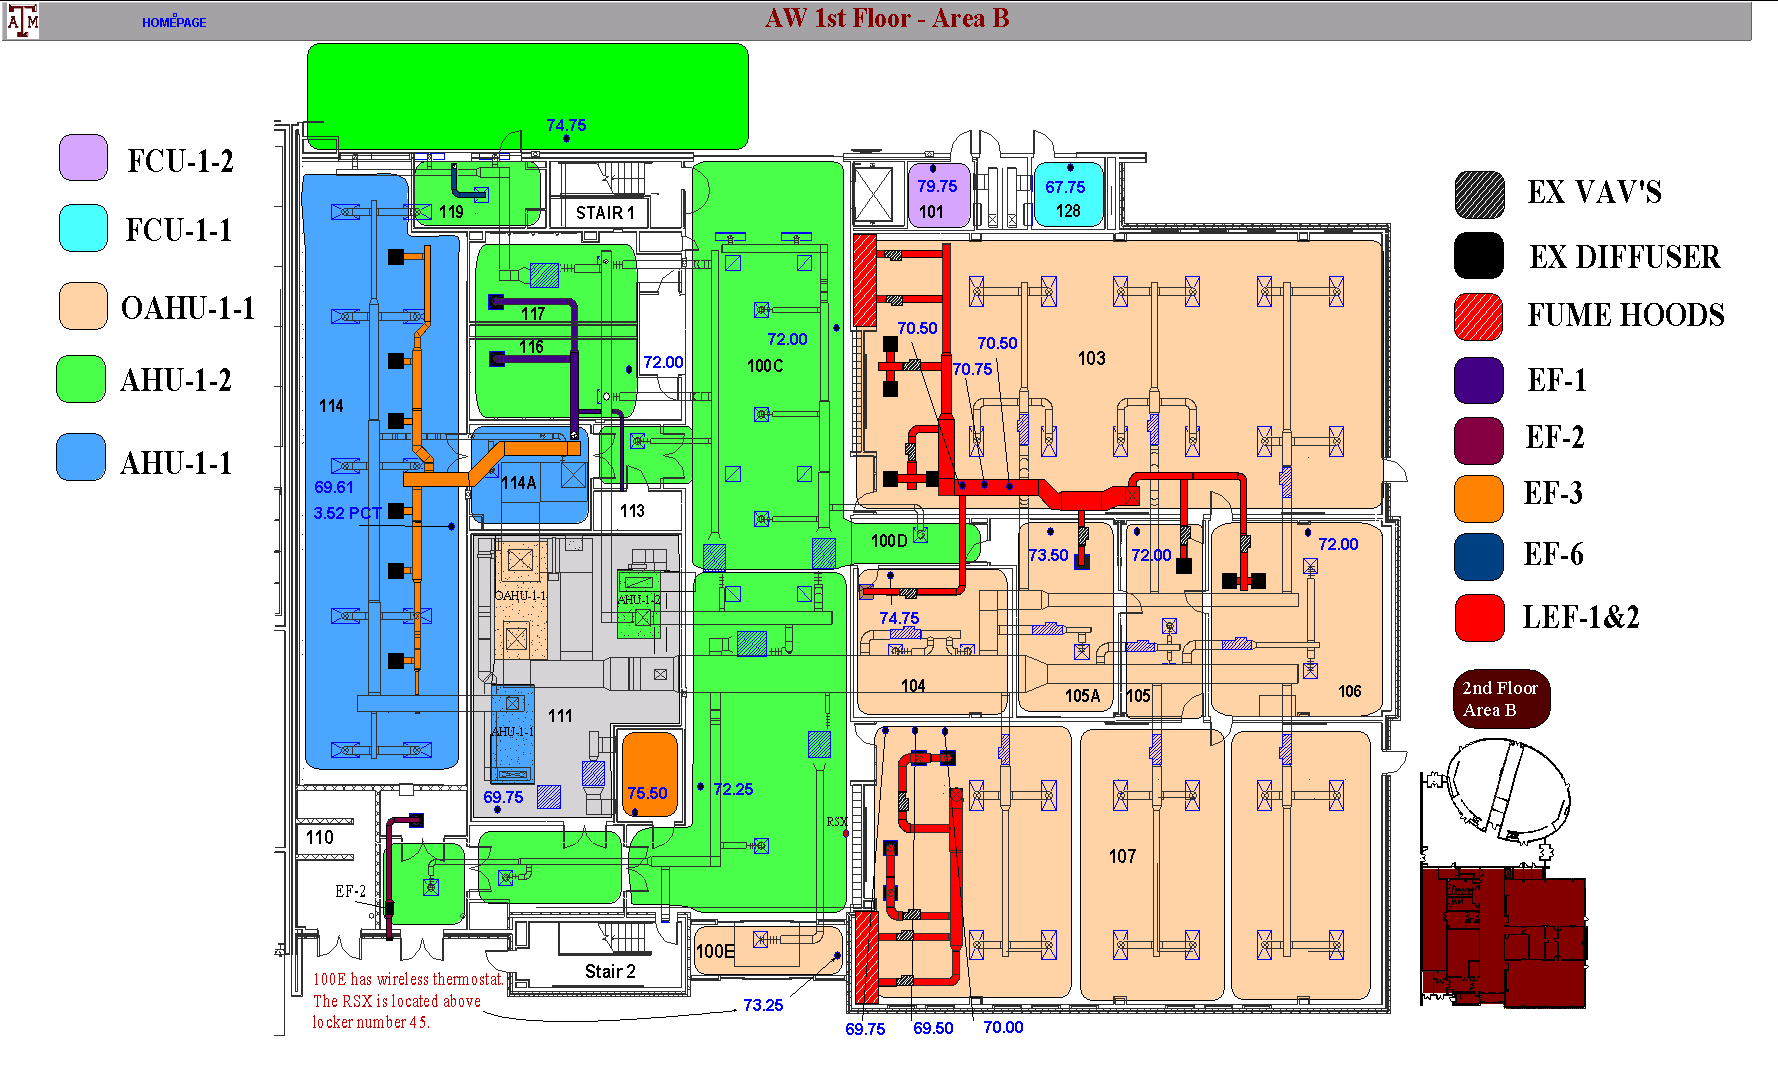
\includegraphics[height=\textwidth]{Images/FirstFloorPlanAreaB.PNG}
        %\caption{First floor plan for Area B.}
        %\label{fig:FirstFloorPlanAreaB}
    %\end{figure}
%\end{landscape}

\begin{figure}
\centering
\includegraphics[width=\textwidth]{Images/SecondFloorPlan.PNG}
\caption{Second floor plan.}
\label{fig:SecondFloorPlan}
\end{figure}

%\begin{landscape}
%\begin{figure}
%\centering
%\includegraphics[height=\textwidth]{Images/SecondFloorPlan.PNG}
%\caption{Second floor plan.}
%\label{fig:SecondFloorPlan}
%\end{figure}
%\end{landscape}


\newcommand{\FloorPlanCaption}[1]{Floor plan for first floor Area #1 with terminal units.}

\begin{figure}
    \centering
    % left, bottom, right, top 
    
\includegraphics[width=\textwidth]{Images/FirstFloorAreaA.pdf}
    \caption{\FloorPlanCaption{A}}
    \label{fig:TerminalUnitLayoutAreaA}
\end{figure}

%\begin{landscape}
    %\begin{figure}
    %\centering
%% left, bottom, right, top 
    %
\includegraphics[totalheight=\textwidth]{Images/FirstFloorAreaA.pdf}
    %\caption{\FloorPlanCaption{A}}
    %\label{fig:TerminalUnitLayoutAreaA}
    %\end{figure}
%\end{landscape}

\begin{figure}
    \centering
    
\includegraphics[width=\textwidth]{Images/FirstFloorAreaB.pdf}
    \caption{\FloorPlanCaption{B}}
    \label{fig:TerminalUnitLayoutAreaB}
\end{figure}

%\begin{landscape}
%\begin{figure}
%\centering
%
\includegraphics[totalheight=\textwidth]{Images/FirstFloorAreaB.pdf}
%\caption{\FloorPlanCaption{B}}
%\label{fig:TerminalUnitLayoutAreaB}
%\end{figure}
%\end{landscape}

\begin{figure}
    \centering
    
\includegraphics[width=\textwidth]{Images/SecondFloorNCTM.pdf}
    \caption{Floor plan for the second floor with terminal units.}
    \label{fig:TerminalUnitLayoutSecondFloor}
\end{figure}

%\begin{landscape}
    %\begin{figure}
        %\centering
        %
\includegraphics[totalheight=\textwidth]{Images/SecondFloorNCTM.pdf}
        %\caption{Floor plan for the second floor with terminal units.}
        %\label{fig:TerminalUnitLayoutSecondFloor}
    %\end{figure}
%\end{landscape}

It is critical to have an understanding of how the current controls     
are operating. It is better to rely on data, rather than relying on     
control code, although in practice, this will normally require that an  
engineer verifies both the control code along with the real measured    
performance.                                                            

\textit{Implementer} can ease the difficulty in this analysis by        
producing certain plots en mass for terminal units. As an example       
of this, \figref{} \ref{fig:TempRise-2-14} shows the results of         
temperature rise within the terminal unit, versus the part-load ratio   
of the terminal unit (assuming the design specifications for the design 
flow). Implementer can produce these plots for every terminal unit in   
a project at once. From these types of plots, the minimum primary air   
flow setpoint can quickly be visually determined.                       

From the data, it appears that the majority of the terminal units       
in NCTM are operating with 30\% as the minimum flow rate. There are     
a few terminal units that have minimum flow rates less than this.       
\tableref{} \ref{tab:MinimumAirFlowRateSettings} shows the estimated    
minimum percent flows based on data from February 1, 2016, through May  
1, 2016.                                                                

\begin{figure}
    \centering
\includegraphics{Plots/TempRiseVsFlow-AHU-2-14.pdf}
\caption{Temperature rise due to the mixing of plenum air at the terminal unit for FPVAV-2-14. Plots like this were used to estimate the current minimum flow rate settings. }
\label{fig:TempRise-2-14}
\end{figure}

\begin{figure}
\centering
\includegraphics[width=\linewidth]{Images/FanPoweredBoxSnip.PNG}
\caption{Typical graphic of the terminal units at NCTM.}
\label{fig:NCTMTerminalUnitGraphic}
\end{figure}

\figref{} \ref{fig:NCTMTerminalUnitGraphic} shows the available points
for the series fan powered terminal units at NCTM from a BAS graphic.

The points include
\begin{itemize}
    \item Primary air flow
    \item Damper command
    \item Discharge air temperature 
    \item Heating coil valve command
\end{itemize}


%% Several unique patterns and characteristics were found in the data set.



%% This information was gathered from the batch plot: 
%% Batch Plots -- Mitch Dissertation N -- 2016-09-21 1347

\begin{table}
\centering
\caption{Terminal unit minimum air flow rate settings.}
\label{tab:MinimumAirFlowRateSettings}
\begin{tabular}{lS}
    \toprule
Terminal Unit & {Min Percent Flow} \\ \midrule
FPVAV-2-1     & 20                 \\
FPVAV-2-2     & 30                 \\
FPVAV-2-3     & 20                 \\
FPVAV-2-12    & 30                 \\
FPVAV-2-13    & 30                 \\
FPVAV-2-14    & 30                 \\
FPVAV-2-15    & 30                 \\
FPVAV-2-16    & 30                 \\
FPVAV-2-17    & 30                 \\
FPVAV-2-18    & 30                 \\
FPVAV-2-9     & 5                  \\
FPVAV-2-10    & 30                 \\
FPVAV-2-11    & 30                 \\
FPVAV-2-4     & 30                 \\
FPVAV-2-5     & 30                 \\
FPVAV-2-6     & 30                 \\
FPVAV-2-7     & 30                 \\
FPVAV-2-8     & 30                 \\
FPVAV-1-10    & 30                 \\
FPVAV-1-7     & 30                 \\
FPVAV-1-8     & {N/A}              \\
FPVAV-1-9     & {N/A}              \\
FPVAV-1-1     & 30                 \\
FPVAV-1-2     & 30                 \\
FPVAV-1-3     & 25                 \\
FPVAV-1-4     & 25                 \\
FPVAV-1-5     & {N/A}              \\
FPVAV-1-6     & 30                 \\
FPVAV-1-11    & 30                 \\ \bottomrule
\end{tabular}
\end{table}





\section{Analysis of the Mixed Air Temperature at the AHU}

This section investigates the feasibility of estimating                 
the mixed air temperature based on historical data. The                 
historical data of the mixed air temperature, \(\mat{}\),               
differs from one air handling unit to another. \figref{}                
\ref{fig:AHU21MixedAirTempvsOADryBulbTemperatureNOAA} shows             
an example of an AHU in which \(\mat\) does not change                  
significantly throughout time, having a range of approximately          
\SI{6}{\degreeF}, excluding a few outliers. In the case of              
\figref{} \ref{fig:AHU13MixedAirTempvsOADryBulbTemperatureNOAA},        
\(\mat\) is less constant but still appears to be a function            
of \(\oat\) as a first order approximation. \figref{}                   
\ref{fig:AHU21MixedAirTempvsOADryBulbTemperatureNOAA} and               
\ref{fig:AHU13MixedAirTempvsOADryBulbTemperatureNOAA} both show data    
spanning 90 days from March 14, 2016 to June 12, 2016.                  



%%These are found in Batch Plots -- Mitch Dissertation N -- 2016-06-13 1354.xlsx batch plot output. 
\begin{figure}
\centering
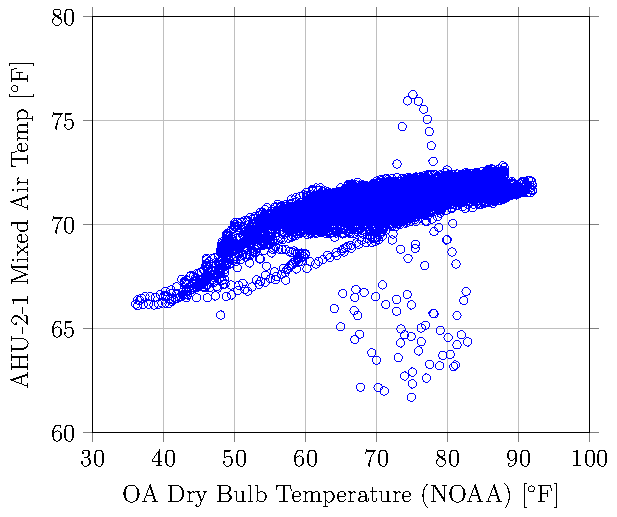
\includegraphics{Plots/2016-06-13-1441-AHU21MixedAirTempvsOADryBulbTemperatureNOAA.pdf}
\caption{AHU-2-1 mixed air temperature vs. outdoor air temperature.}
\label{fig:AHU21MixedAirTempvsOADryBulbTemperatureNOAA}
\end{figure}


\begin{figure}
\centering
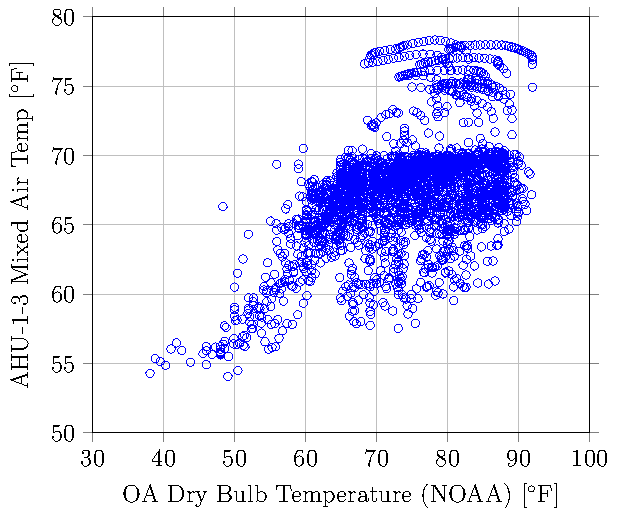
\includegraphics{Plots/2016-06-13-1459-AHU13MixedAirTempvsOADryBulbTemperatureNOAA.pdf}
\caption{AHU-1-3 mixed air temperature vs. outdoor air temperature.}
\label{fig:AHU13MixedAirTempvsOADryBulbTemperatureNOAA}
\end{figure}

The \textit{nearest neighbor} approach was used to predict the mixed air
temperatures. The algorithm looked
back in history (at least a day before) under the following parameters:

\begin{itemize}
    \item The same day of the week (Sun, Mon, etc.)
    \item Same hour of day \(\pm\)1 hr.
    \item Same \(\oat{}\) \(\pm\)3\(^\circ\)F
    \item Searching backward until 30 data points found
\end{itemize}



The median of the data points matching the criterion                    
listed is the resulting predicted value. \figref{}                      
\ref{fig:2016-09-07-1218-AHU12MixedAirTempvsOADryBulbTemperatureNOAA}   
and \ref{fig:AHU13MixedAirTempvsOADryBulbTemperatureNOAA-2}             
show the results versus outdoor air temperature. The following          
plots show the model fits for the different air handling                
units at NCTM. The data covers a period of 180 days. Figures            
\ref{fig:2016-09-07-1218-AHU12MixedAirTempvsOADryBulbTemperatureNOAA}   
and \ref{fig:AHU13MixedAirTempvsOADryBulbTemperatureNOAA-2} show that   
the prediction algorithm can adequately handle the differences from     
when the air handling unit is on as well as off. The significant amount 
of spread in the mixed air temperature is due to data in which the      
air handler turns off and is allowed to drift, typically to a higher    
temperature in the climate of College Station.                          

Figures
\ref{fig:2016-09-07-1335-MixedAirTempPredictionforAHU12vsAHU12MixedAirTemp}
through
\ref{fig:2016-09-07-1623-MixedAirTempPredictionforAHU23vsAHU23MixedAirTemp}
show the model fits ignoring times when the air handling units are off,
weekends and holidays, and times between 6:00 PM and 8:00 AM.

\newcommand{\matcaption}[1]{#1 \(\mat\) prediction for data from March 10, 2016 - September 5, 2016, not ignoring any data.}

\begin{figure}
\centering
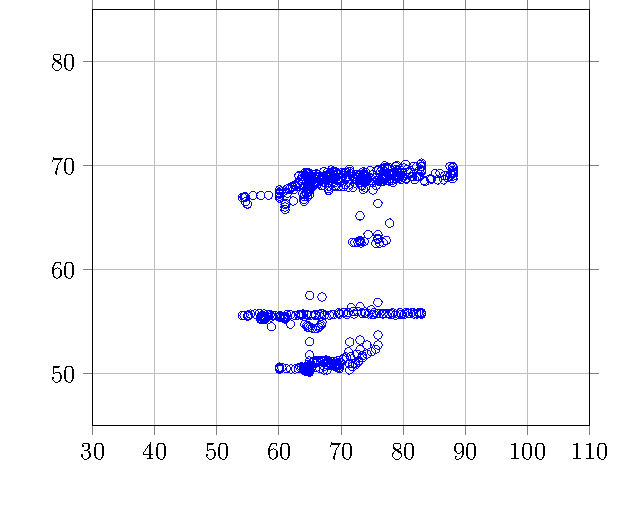
\includegraphics{Plots/2016-09-07-1218-AHU12MixedAirTempvsOADryBulbTemperatureNOAA.pdf}
\caption{\matcaption{AHU-1-2}}
\label{fig:2016-09-07-1218-AHU12MixedAirTempvsOADryBulbTemperatureNOAA}
\end{figure}

\begin{figure}
\centering
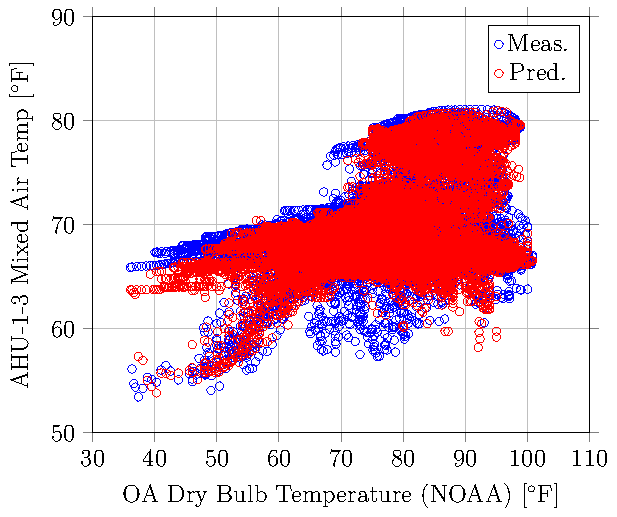
\includegraphics{Plots/2016-09-07-0943-AHU13MixedAirTempvsOADryBulbTemperatureNOAA.pdf}
\caption{AHU-1-3 mixed air temperature prediction for data from March 10, 2016 - September 5, 2016, not ignoring any data.}
\label{fig:AHU13MixedAirTempvsOADryBulbTemperatureNOAA-2}
\end{figure}



%% 45 degree plots showing the adequacy of the model fit. 

\newcommand{\mixAirCaptionTwo}[1]{Mixed air temperature prediction results for #1.}

\begin{figure}
\centering
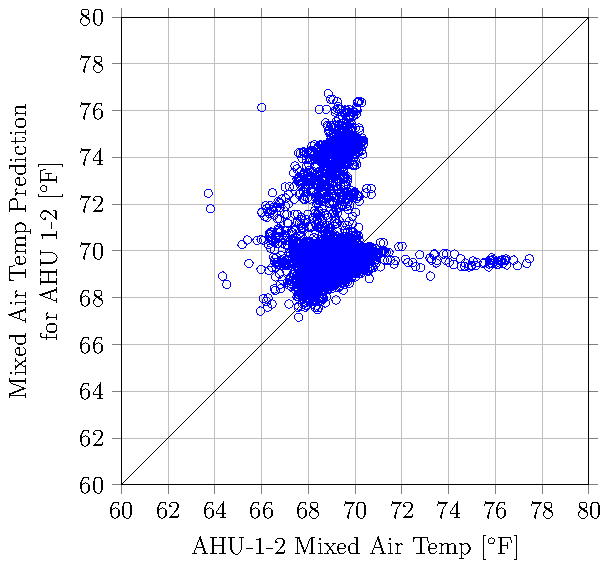
\includegraphics{Plots/2016-09-07-1335-MixedAirTempPredictionforContainerAHU12vsAHU12MixedAirTemp.pdf}
\caption{\mixAirCaptionTwo{AHU-1-2}}
\label{fig:2016-09-07-1335-MixedAirTempPredictionforAHU12vsAHU12MixedAirTemp}
\end{figure}

\begin{figure}
\centering
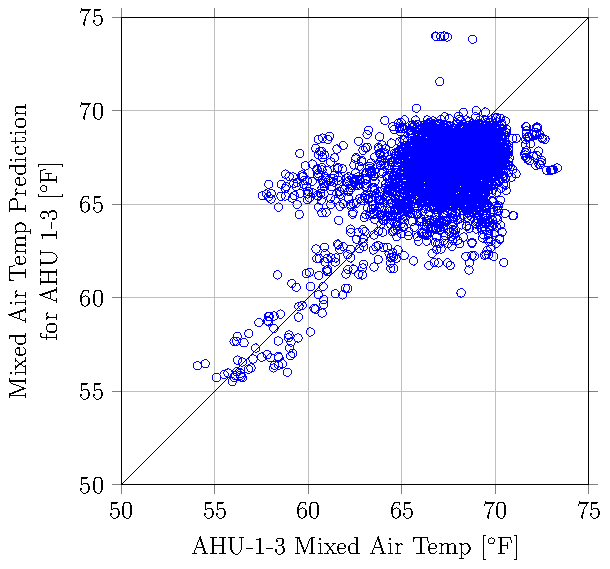
\includegraphics{Plots/2016-09-07-1346-MixedAirTempPredictionforContainerAHU13vsAHU13MixedAirTemp.pdf}
\caption{\mixAirCaptionTwo{AHU-1-3}}
\label{fig:2016-09-07-1346-MixedAirTempPredictionforContainerAHU13vsAHU13MixedAirTemp}
\end{figure}

\begin{figure}
\centering
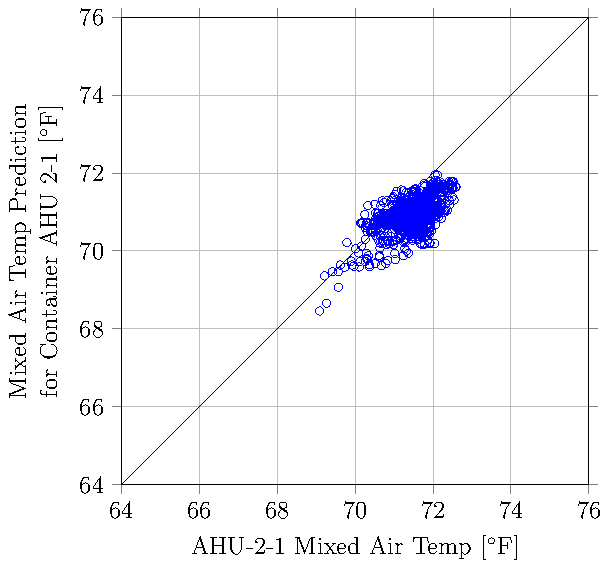
\includegraphics{Plots/2016-09-07-1357-MixedAirTempPredictionforContainerAHU21vsAHU21MixedAirTemp.pdf}
\caption{\mixAirCaptionTwo{AHU-2-1}}
\label{fig:2016-09-07-1357-MixedAirTempPredictionforContainerAHU21vsAHU21MixedAirTemp}
\end{figure}

\begin{figure}
\centering
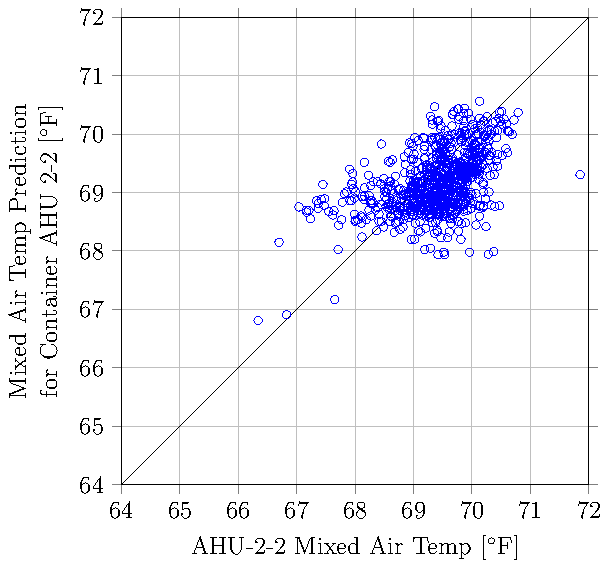
\includegraphics{Plots/2016-09-07-1619-MixedAirTempPredictionforContainerAHU22vsAHU22MixedAirTemp.pdf}
\caption{\mixAirCaptionTwo{AHU-2-2}}
\label{fig:2016-09-07-1619-MixedAirTempPredictionforContainerAHU22vsAHU22MixedAirTemp}
\end{figure}

\begin{figure}
\centering
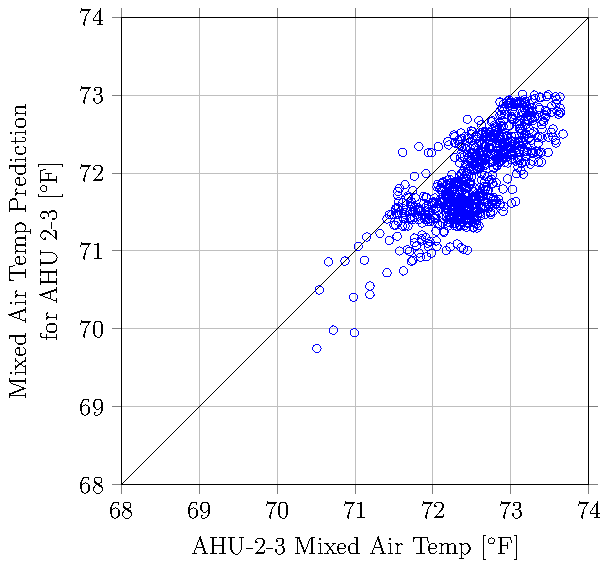
\includegraphics{Plots/2016-09-07-1623-MixedAirTempPredictionforContainerAHU23vsAHU23MixedAirTemp.pdf}
\caption{\mixAirCaptionTwo{AHU-2-3}}
\label{fig:2016-09-07-1623-MixedAirTempPredictionforAHU23vsAHU23MixedAirTemp}
\end{figure}


The sensitivity of the prediction results to the selected nearest       
neighbor parameters was tested. The parameter values were varied as     
shown in \tableref{} \ref{tab:NearestNeighborVariations}.               

\begin{table}
\centering
\caption{Variations in the parameters for the nearest neighbor algorithm.}
\label{tab:NearestNeighborVariations}
\begin{tabular}{rl}
    Threshold & Variations \\ \midrule
    Time stamp threshold & 15, 30, and 60 minutes \\
    \(T_{oa} \) threshold & \SI{1}{\degF}, \SI{3}{\degF}, \SI{5}{\degF} \\
    Data points threshold & 15, 30, and 45 data points. 
\end{tabular}
\end{table}


With three parameters and three different variations for each, this resulted
in 27 test cases. The results of this testing are shown in \tableref{}
\ref{tab:MATTestingResults}. TS stands for timestamps and is related to
the time of day threshold. Since the data was aligned to 15 minute
intervals, a 1 timestamp threshold implies a threshold of \(\pm\)15
minutes and a 4 timestamp threshold implies a threshold of \(\pm\)60
minutes. The best model fit used a timestamp threshold of \(\pm\)60
minutes, \(\pm\SI{3}{\degF}\) for \(T_{oa}\), and 15 data points. The
worst case was using \(\pm\)15 minutes, \(\pm \SI{1}{\degF}\), and 30
data points. 

 Because Fahrenheit is not on a ratio scale, that is, having a
 meaningful zero, the typical goodness-of-fit parameter, the coefficient
 of variation of the root mean squared error (RMSE), has less meaning.
 Therefore, instead of using the mean as the normalization parameter in
 the CV-RMSE metric, the range or the spread of the original data was
 used. It is denoted as CV-RMSE* for the remainder of this document. 

\begin{equation}\label{eq:CVRMSEStar}
\text{CV-RMSE*} = \frac{\text{RMSE}}{y_{max}-y_{min}}
\end{equation}

The model was insensitive to the parameters. The average CV-RMSE*       
ranged from 8.97\% to 10.75\% across the 27 different test cases. The   
models with the lowest CVs had the largest range in the timestamp and   
\(T_{oa}\) threshold. This observation is an indication that using more 
recent data was more valuable than using data from conditions matching  
more closely, though the more important fact was that the overall       
difference from highest to lowest CV-RMSE* was only 1.78 percentage     
points.                                                                 

A graphical view of the results in order of the best set parameters to
the worst set of parameters is shown in \figref{}
\ref{fig:MATPredictionOrderedResults}. 

\begin{table}
    \centering
    \caption{Results from testing different nearest neighbor model
    parameters for predicted \(\mat{}\).}
    \label{tab:MATTestingResults}
    \begin{tabular}{@{}llllS[round-mode=off,table-format=2.2]@{}}
        \toprule
        Run & TS & \(T_{oa}\) & DP & { Average CV-RMSE* }\\ \midrule
        1   & 1  & 1          & 15 & 10.12      \\
        2   & 2  & 1          & 15 & 9.68       \\
        3   & 4  & 1          & 15 & 9.80       \\
        4   & 1  & 3          & 15 & 9.61       \\
        5   & 2  & 3          & 15 & 9.41       \\
        6   & 4  & 3          & 15 & 8.97       \\
        7   & 1  & 5          & 15 & 9.28       \\
        8   & 2  & 5          & 15 & 9.18       \\
        9   & 4  & 5          & 15 & 8.98       \\
        10  & 1  & 1          & 30 & 10.58      \\
        11  & 2  & 1          & 30 & 10.07      \\
        12  & 4  & 1          & 30 & 9.39       \\
        13  & 1  & 3          & 30 & 9.95       \\
        14  & 2  & 3          & 30 & 9.63       \\
        15  & 4  & 3          & 30 & 9.16       \\
        16  & 1  & 5          & 30 & 9.61       \\
        17  & 2  & 5          & 30 & 9.25       \\
        18  & 4  & 5          & 30 & 9.00       \\
        19  & 1  & 1          & 45 & 10.75      \\
        20  & 2  & 1          & 45 & 10.47      \\
        21  & 4  & 1          & 45 & 9.80       \\
        22  & 1  & 3          & 45 & 10.08      \\
        23  & 2  & 3          & 45 & 9.58       \\
        24  & 4  & 3          & 45 & 9.32       \\
        25  & 1  & 5          & 45 & 9.74       \\
        26  & 2  & 5          & 45 & 9.52       \\
        27  & 4  & 5          & 45 & 9.08       \\ \bottomrule
    \end{tabular}
\end{table}

\begin{figure}
\centering
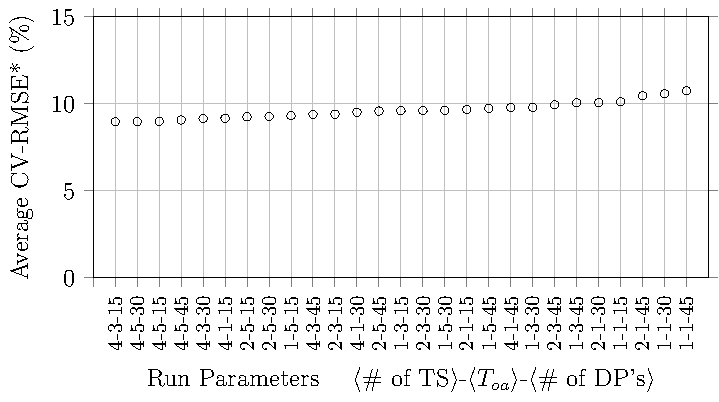
\includegraphics{Plots/03/2017-06-08-MATPredOrder.pdf}
\caption{Results from testing different nearest neighbor model
parameters used in predicting mixed air temperature. }
\label{fig:MATPredictionOrderedResults}
\end{figure}


\sisetup{round-mode=figures, round-precision=3}

\begin{table}
\centering
\caption{\(\mat{}\) prediction results using the parameters in Run 6.}
\label{tab:MATPredictionResultsForRun6}
\begin{tabular}{lS} \toprule
    AHU     & {RMSE (\si{\degF})  } \\ \midrule
    AHU 1-2 & 1.686834982  \\
    AHU 1-3 & 2.41776849   \\
    AHU 1-4 & 1.251856851   \\
    AHU 2-1 & 0.744179046   \\
    AHU 2-2 & 0.619408965   \\
    AHU 2-3 & 0.495786538   \\ \bottomrule
\end{tabular}
\end{table}

\section{Analysis of the Plenum Air Temperature}

Reheat is a major component of energy use, and for a series fan powered
box, the plenum air temperature is required to calculate the reheat
power.  This section analyzes the estimation of the plenum air
temperature and the corresponding uncertainty.  If the terminal unit is
modeled as a simple mixing problem, with negligible impact from the fan,
the plenum air temperature will be 
\begin{equation}\label{eq:PlenumTemperatureSimpleMixing}
    T_{plen}=\frac{\flow{tot}T_{dis}-\flow{pri}\sat{}}{\flow{tot} -\flow{pri}}
\end{equation}

Since \(T_{plen}\) is a function of 4 variables, each with their        
own uncertainties, it is important to consider the cumulative           
uncertainty in the estimation. Clearly, when \(\flow{plen}\) (or        
\(\flow{tot} - \flow{pri}\), the denominator of \eqreftext{}            
\ref{eq:PlenumTemperatureSimpleMixing}) is low, the uncertainty in      
\(T_{plen}\) grows significantly, and when the flow is equal to zero,
\(T_{plen}\) is undefined.                                              

Using the Kline-McKlintock formulation of uncertainty, the uncertainty
of \(T_{plen}\) is 

\begin{multline}
    \delta T_{plen} = \left[\left( \pdv{T_{plen}}{\flow{pri}} \delta \flow{pri}   \right)^2  +\left( \pdv{T_{plen}}{\flow{tot}} \delta \flow{tot}   \right)^2 + \right. \\
    \left. \left( \pdv{T_{plen}}{T_{dis}} \delta T_{dis}   \right)^2 + \left( \pdv{T_{plen}}{\sat{}} \delta \sat{}   \right)^2  \right]^{1/2}
\end{multline}

\begin{multline}\label{eq:plenumUncertainty}
    \delta T_{plen} = \left[\left(  \frac{\flow{tot}\left(T_{dis}-\sat{}
    \right)}{{\flow{plen}}^2}   \delta \flow{pri} \right)^2
+\left(\frac{\flow{pri}\left(\sat{}-T_{dis} \right)}{{\flow{plen}}^2}      \delta \flow{tot}   \right)^2 + \right. \\
    \left. \left( \frac{\flow{tot}}{\flow{plen}} \delta T_{dis}
    \right)^2 + \left(\frac{\flow{pri}}{\flow{plen}}  \delta \sat{}   \right)^2  \right]^{1/2}
\end{multline}

As a concrete example, if the following arbitrary but reasonable parameters are used, 
%
\newcommand{\flowtotvalue}{\SI{2200}{\CFM}}
\newcommand{\plenflowvalue}{\SI{1000}{\CFM}}
%
\begin{itemize}
    \item \(\totflow{}=\flowtotvalue\)
    \item \(\priflow{}=\plenflowvalue\)
    \item \(\plenflow=\flowtotvalue - \plenflowvalue = \SI{1200}{\CFM} \)
    \item \(\sat = 55^{\circ}\text{F} \)
    \item \(\dat = 75^{\circ}\text{F} \)
    \item \(\delta\priflow{}=\delta\plenflow=\delta\totflow=100 \text{ CFM}\)
    \item \(\delta \sat = \delta \dat = 1^{\circ} \text{F} \)
\end{itemize}
%
Equation \ref{eq:plenumUncertainty} becomes
\begin{equation}\label{eq:plenumUncertainty2}
    \delta T_{plen} = \left[\left(  \SI{3.06}{\degreeF}  \right)^2  +\left( \SI{-1.39}{\degreeF}  \right)^2 +  \left( \SI{1.83}{\degreeF} \right)^2 + \left(\SI{0.83}{\degreeF}  \right)^2  \right]^{1/2}
\end{equation}
which results in a final uncertainty of \SI{3.91}{\degreeF}, which is
nearly four times larger than the initially assumed uncertainties for
the temperatures (\SI{1}{\degreeF}). When \(\flow{plen}\) is reduced even
further, this uncertainty grows substantially.  

For a more detailed analysis, \eqreftext{} \ref{eq:plenumUncertainty}   
can be manipulated into a simpler form. The first substitution          
assumes the uncertainty for \(T_{dis}\) and \(T_{pri}\) are the same    
and constant at a value of \(\delta T\). The uncertainty of the         
flows can be done on a percent basis (\(\pm 10\%\) for example, and     
that percentage, a value from 0 to 1, can be denoted as \(\delta        
\flow{perc}\)). The difference between \(T_{dis}\) and \(T_{pri}\)      
can be replaced by \(\Delta T\). The final substitution is that the     
flows for \(\flow{pri}\) and \(\flow{plen}\) are replaced by the        
corresponding fraction of the total flow. \(F_{pri}\) is defined to be  
the fraction of the total flow that comes from the primary stream, a    
value between 0 and 1. Therefore, 
\begin{equation} 
    \Delta T = T_{dis} - T_{pri}
\end{equation}
and 
\begin{equation} 
    \flow{pri} = F_{pri} \flow{tot}
\end{equation} 
and 
\begin{equation} 
    \flow{plen} = \left(1- F_{pri}\right) \flow{tot}. 
\end{equation} 
With these substitutions, the total uncertainty for \(T_{plen}\) is 
\begin{equation}              
    \sqrt{\left(\frac{\delta T}{1-F_{pri}}\right)^2 + \left(\frac{\delta    
    T F_{pri}}{1-F_{pri}}\right)^2 + 2 \left(\frac{\Delta T\,               
    F_{pri}\,\delta\flow{perc} } {(1-F_{pri})^2}\right)^2}
\end{equation}

Various combinations of values and the resulting uncertainty in
\(T_{plen}\) are shown in \figref{}
\ref{fig:TPlenUncertaintyAcrossDeltaT} through
\ref{fig:TPlenUncertaintyAcrossVUnc}. The y-axis is normalized to the
static uncertainty in the other temperatures, \(\delta T\), which is the
uncertainty for both \(T_{dis} \) and \(T_{pri}\). 

What the plots show is that the fraction of primary flow, \(F\), has to
be less than 40\% in most cases to have an uncertainty in
\(T_{plen}\) that is less than double the uncertainty in \(T_{dis}\) and
\(T_{pri}\) (a value of 2 on the normalized y-axis). 


% Plots/2017-06-07-TplenUncertainty.tex
\begin{figure}
\centering
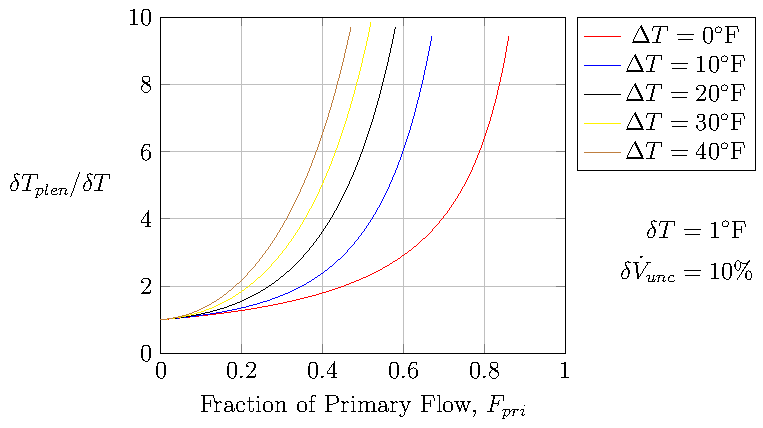
\includegraphics{Plots/2017-06-07-TplenUncertainty.pdf}
\caption{Uncertainty in \(T_{plen}\), \(\delta T_{plen}\), at different
levels of \(\Delta T = T_{dis} - T_{pri}\). }
\label{fig:TPlenUncertaintyAcrossDeltaT}
\end{figure}

% Plots/2017-06-07-TPlenumUncVaryDelT.tex
\begin{figure}
\centering
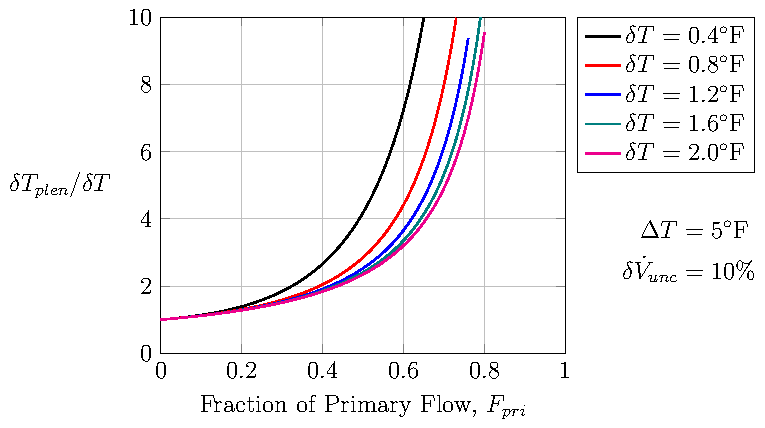
\includegraphics{Plots/2017-06-07-TPlenumUncVaryDelT.pdf}
\caption{Uncertainty in \(T_{plen}\), \(\delta T_{plen}\), at different levels of \(\delta T\). }
\label{fig:TPlenUncertaintyAcrossdelT}
\end{figure}

% Plots/2017-06-07-TPlenumUncVaryVUnc.tex
\begin{figure}
\centering
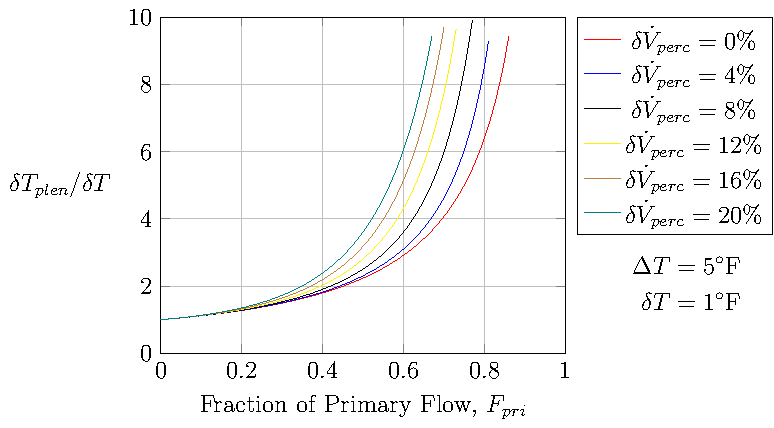
\includegraphics{Plots/2017-06-07-TPlenumUncVaryVUnc.pdf}
\caption{Uncertainty in \(T_{plen}\), \(\delta T_{plen}\), at different levels of \(\delta \flow{unc}\). }
\label{fig:TPlenUncertaintyAcrossVUnc}
\end{figure}

As an example as to how unstable the calculation for the plenum
temperature is, \figref{}
\ref{fig:2016-09-16-1006-PlenumTemperatureforContainerFPVAV19vsZoneLoadforContainerFPVAV19}
shows the calculated plenum temperature for FPVAV-1-9 over the period
from February 1, 2016 - May 1, 2016. The calculated values are
unrealistic ranging from -1,500\(^\circ\)F to 1,500\(^\circ\)F. The
reason for this is made clear in a time series plot of the flows related
to the terminal unit. As shown in \figref{}
\ref{fig:2016-09-16-1639-FPVAV19AIRVOLUME-TikzData}, for this particular
terminal unit, the primary flow is either near zero or design. At times,
the measured flow is also above the design specification, making the
plenum flow calculation zero. When the plenum flow is calculated to be
zero, the plenum temperature calculation becomes undefined.                                                      

Using the assumptions that the uncertainty in the flow was 100 CFM      
and the uncertainty in the temperature measurements was 1\(^\circ\)F,   
the plenum temperature was calculated from October 6, 2015, to          
September 12, 2016, ignoring items that appear in \tableref{}           
\ref{tab:PlenumTemperatureEstimation}. The distribution statistics for  
each terminal unit are found in \tableref{} \ref{tab:plenumStatistics}. 
The table is listed in ascending order by the median of the plenum      
temperature calculated.                                                 

Note that the percentage of ignored points is below 96\% for only 4     
terminal units. The majority of the points are ignored because the      
uncertainty in the calculation was above the 2\(^\circ\)F threshold     
that was arbitrarily chosen. In fact, at no point was the uncertainty   
below 2\(^\circ\)F for FPVAV-2-7. The median plenum temperature ranges  
from 58.8\(^\circ\)F for FPVAV-1-8 to 75.6\(^\circ\)F for FPVAV-1-6.    

Another interesting way to examine the difference between the plenum
temperature and the zone temperature is to plot the estimated reheat in
the terminal unit when the reheat valve is closed.  Ideally, the amount
of reheat would be at or near zero. 

If the plenum temperature is assumed to be equal to the zone
temperature, then an estimate of the mixed air temperature in the
terminal unit would be
\begin{equation}
    \mat = \frac{\priflow \sat + T_{z} \left( \totflow - \priflow \right) }{ \totflow}
    \label{eq:TerminalUnitMixedAirTemp}
\end{equation}
and the reheat power could be estimated by
\begin{equation}
    \heatenergy{} = 1.08 \left( CFM \right) \left( \mat - \dat  \right)
    \label{eq:TerminalUnitReheatEnergy}
\end{equation}

\figref{}s
\ref{fig:2016-10-19-1424-ZoneReheatEnergyforContainerFPVAV216vsOADryBulbTemperatureNOAA}
through
\ref{fig:2016-10-19-1521-ZoneReheatEnergyforContainerFPVAV213vsOADryBulbTemperatureNOAA}
show the reheat power as determined by \eqreftext{}
\ref{eq:TerminalUnitReheatEnergy}. They are from the period of February
1, 2016, through May 1, 2016.  Timestamps during weekends, times between
5:00 PM and 9:00 AM, and when the corresponding reheat valve command is
\( <1\%\) were ignored. Again, ideally, the estimated reheat power would
be exactly zero.


\begin{table}
\centering
\caption{Implementer settings for plenum temperature estimation for NCTM, used to calculate data in \tableref{} \ref{tab:plenumStatistics}.}
\label{tab:PlenumTemperatureEstimation}
\begin{tabular}{@{}rl@{}}
\toprule
Project:            & Mitch Dissertation NCTM---2016-09-19 10:34           \\ \midrule
Scope:              & NCTM                                                 \\
Axis Parameters:    & Plenum Temperature vs. OA Dry-bulb Temp (NOAA)       \\
Date Period:        & 10/6/2015 - 9/12/2016  (342 days)                    \\
OAT range:          & 31 to 100\(^\circ\)F                                 \\
Ignoring:           & When AHU is Off                                      \\
                    & First 1.0 hours of operation                         \\
                    & Last 1.0 hours of operation                          \\
                    & Sundays                                              \\
                    & Saturdays                                            \\
                    & Federal Holidays                                     \\
                    & Hours from 17:00 to 9:00                             \\
                    & When label Plenum Temp Uncertainty is greater than 2 \\
                    & When label Valve Positions is greater than 1         \\ \bottomrule
\end{tabular}
\end{table}


%Plots/2016-09-16-1006-PlenumTemperatureforContainerFPVAV19vsZoneLoadforContainerFPVAV19.tex
\begin{figure}
\centering

\includegraphics{Plots/2016-09-16-1006-PlenumTemperatureforContainerFPVAV19vsZoneLoadforContainerFPVAV19.pdf}
\caption{Calculated plenum temperature for FPVAV-1-9.}
\label{fig:2016-09-16-1006-PlenumTemperatureforContainerFPVAV19vsZoneLoadforContainerFPVAV19}
\end{figure}

\begin{figure}
\centering
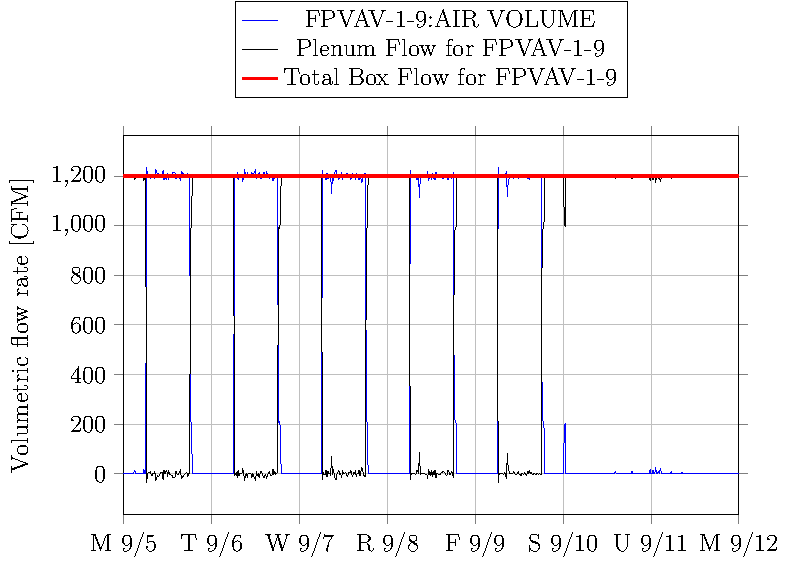
\includegraphics{Plots/2016-09-16-1639-FPVAV19AIRVOLUME-TikzData.pdf}
\caption{Flowrates for FPVAV-1-9.}
\label{fig:2016-09-16-1639-FPVAV19AIRVOLUME-TikzData}
\end{figure}




%Project:	Mitch Dissertation NCTM---2016-09-19 10:34
%Scope:	NCTM
%Axis Parameters:	Plenum Temperature vs. OA Drybulb Temp (NOAA)
%Date Period:	10/6/2015 - 9/12/2016  (342 days)
%OAT range:	31 to 100 �F
%Ignoring:	When AHU is Off
	%First 1.0 hours of operation
	%Last 1.0 hours of operation
	%Sundays
	%Saturdays
	%Federal Holidays
	%Hours from 17:00 to 9:00
	%When label Plenum Temp Uncertainty is greater than 2
	%When label Valve Positions is greater than 1

\begin{table}
\centering
\caption{Calculated plenum temperature statistics for NCTM.}
\label{tab:plenumStatistics}
\begin{tabular}{@{}llllllllS[round-mode=off,table-format=5.0]lS[round-mode=off,table-format=4.0]@{}}
    \toprule
    Unit     & Min  & \parbox{1cm}{5th \\ Perc.} & Mean & Median & \parbox{1cm}{95th \\ Perc.} & Max   & \parbox{1cm}{St. \\ Dev. }      & { \parbox{1cm}{Original \\ Count} } & \parbox{1 cm}{\% \\ Ignored } & { \parbox{1cm}{Final \\ Count} }   \\ \midrule
1-8  & 56.5 & 56.5 & 60.6 & 58.8 & 71.8 & 71.8 & 4.25 & 29199 & 99.911\%  &  26         \\
2-12 & 52.8 & 55.7 & 60.8 & 61.8 & 62.5 & 75.0 & 2.23 & 29319 & 88.062\%  &  3500       \\
2-15 & 52.1 & 57.4 & 61.3 & 61.8 & 62.6 & 78.5 & 1.84 & 29324 & 78.645\%  &  6262       \\
1-9  & 57.0 & 57.0 & 63.6 & 65.0 & 73.5 & 73.8 & 5.34 & 27961 & 99.939\%  &  17         \\
2-6  & 65.0 & 65.0 & 65.0 & 65.0 & 65.0 & 65.0 & 0.00 & 29311 & 99.997\%  &  1          \\
2-18 & 61.5 & 62.7 & 69.6 & 67.0 & 80.2 & 80.5 & 5.60 & 29312 & 99.846\%  &  45         \\
2-16 & 67.0 & 67.0 & 67.3 & 67.5 & 67.5 & 67.5 & 0.29 & 29325 & 99.990\%  &  3          \\
2-10 & 66.5 & 66.5 & 67.8 & 67.8 & 69.0 & 69.0 & 1.44 & 29236 & 99.986\%  &  4          \\
2-14 & 60.0 & 61.0 & 68.8 & 68.5 & 79.0 & 79.8 & 6.28 & 29318 & 99.860\%  &  41         \\
2-11 & 66.5 & 66.5 & 68.0 & 68.5 & 69.5 & 69.5 & 1.01 & 28557 & 99.958\%  &  12         \\
2-5  & 68.5 & 68.5 & 69.1 & 69.0 & 70.0 & 70.0 & 0.65 & 29309 & 99.983\%  &  5          \\
2-8  & 68.2 & 69.1 & 70.0 & 70.0 & 70.7 & 72.5 & 0.55 & 29304 & 98.601\%  &  410        \\
2-13 & 68.0 & 68.5 & 70.0 & 70.0 & 71.5 & 72.6 & 1.34 & 29312 & 99.887\%  &  33         \\
1-5  & 55.0 & 63.8 & 71.1 & 70.1 & 78.0 & 79.0 & 4.62 & 30170 & 99.450\%  &  166        \\
2-17 & 61.5 & 68.5 & 70.3 & 70.4 & 71.5 & 72.5 & 1.23 & 29287 & 99.126\%  &  256        \\
2-2  & 52.5 & 67.3 & 70.7 & 70.8 & 73.6 & 75.6 & 2.69 & 29363 & 98.685\%  &  386        \\
1-7  & 60.0 & 64.5 & 71.8 & 71.8 & 75.1 & 75.7 & 3.11 & 29955 & 99.222\%  &  233        \\
2-3  & 64.5 & 71.0 & 73.0 & 72.8 & 75.3 & 76.2 & 1.49 & 29367 & 96.391\%  &  1060       \\
1-2  & 67.0 & 70.8 & 73.9 & 72.9 & 77.8 & 78.5 & 2.60 & 30166 & 99.589\%  &  124        \\
2-1  & 67.5 & 70.8 & 73.6 & 73.8 & 75.5 & 81.7 & 1.44 & 29366 & 96.016\%  &  1170       \\
1-3  & 71.4 & 72.6 & 74.2 & 74.4 & 75.4 & 76.9 & 0.94 & 30145 & 98.202\%  &  542        \\
2-9  & 69.0 & 70.7 & 73.9 & 74.5 & 76.5 & 78.4 & 1.88 & 29272 & 76.356\%  &  6921       \\
1-1  & 57.0 & 71.8 & 74.6 & 74.8 & 79.0 & 82.5 & 2.64 & 30152 & 97.652\%  &  708        \\
1-10 & 58.5 & 62.0 & 73.8 & 74.9 & 76.0 & 78.2 & 3.61 & 29941 & 99.008\%  &  297        \\
1-4  & 54.0 & 72.4 & 74.9 & 75.1 & 77.2 & 81.7 & 2.51 & 30086 & 98.488\%  &  455        \\
2-4  & 69.5 & 73.7 & 75.3 & 75.2 & 76.7 & 77.6 & 0.96 & 29304 & 86.916\%  &  3834       \\
1-6  & 56.5 & 66.2 & 74.1 & 75.6 & 81.3 & 81.6 & 5.43 & 30170 & 99.738\%  &  79         \\
2-7  & N/A  & N/A  & N/A  & N/A  & N/A  & N/A  & N/A  & 28906 & 100.000\% &  0          \\ \bottomrule
\end{tabular}
\end{table}

% For series fan powered terminal units, the assumption was made that the total
% flow remains constant and that the mixed air temperature at the
% individual terminal unit can be predicted based on the primary flow value that is
% measured. 

% One possible assumption for the plenum temperature is that it is equal to the
% corresponding zone temperature. An interesting analysis is then to calculate
% the mixed air temperature based on this assumption and then look at times when
% the reheat valve is commanded to zero. It would be expected that the calculated
% reheat would be near zero, if not slightly above zero due to leakage in the
% reheat valve.  The next series of plots look at data from February 1, 2016 to
% May 1, 2016, ignoring when the unit is off, weekends and holidays, and when the
% commanded reheat coil position is greater than 1\%. 

\figref{}
\ref{fig:2016-10-19-1424-ZoneReheatEnergyforContainerFPVAV216vsOADryBulbTemperatureNOAA}
shows an example of where the assumption appears to hold reasonably well.  
The median of the data set is near \SI{500}{\btu\per\hour}. Is should be
noted that \eqreftext{} \ref{eq:TerminalUnitReheatEnergy} does not make a
distinction between heating from the heating coils and heating from the fan.
So the \SI{500}{\btu\per\hour} could be due to the fan in the air
stream. 

\figref{}
\ref{fig:2016-10-19-1438-ZoneReheatEnergyforContainerFPVAV24vsOADryBulbTemperatureNOAA}
shows a case in which there is either constant reheat or the actual
plenum temperature is lower than the zone temperature that was assumed.

\figref{}
\ref{fig:2016-10-19-1521-ZoneReheatEnergyforContainerFPVAV213vsOADryBulbTemperatureNOAA}
shows a case in which the reheat is estimated to be a negative value,
which likely means that the actual plenum temperature is greater than
the assumed plenum temperature equal to the zone temperature. 



\newcommand{\zoneReheatCaption}[1]{Zone reheat power for terminal unit #1.}

% Plots/2016-10-19-1424-ZoneReheatEnergyforContainerFPVAV216vsOADryBulbTemperatureNOAA.tex
\begin{figure}
\centering
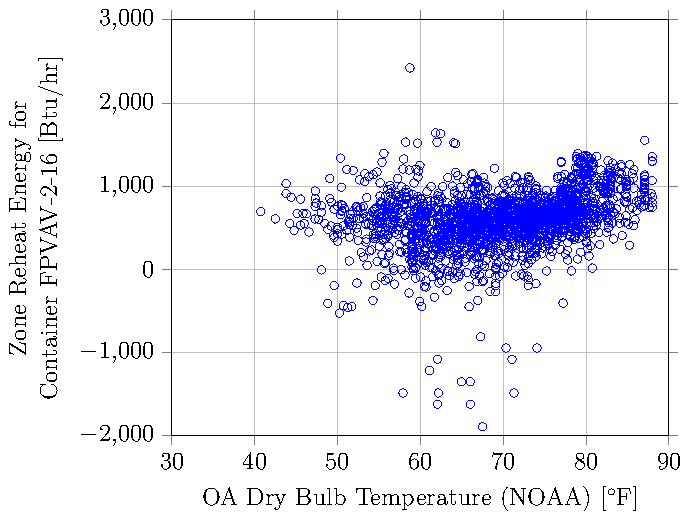
\includegraphics{Plots/2016-10-19-1424-ZoneReheatEnergyforContainerFPVAV216vsOADryBulbTemperatureNOAA.pdf}
\caption{\zoneReheatCaption{2-16}}
\label{fig:2016-10-19-1424-ZoneReheatEnergyforContainerFPVAV216vsOADryBulbTemperatureNOAA}
\end{figure}

% Plots/2016-10-19-1438-ZoneReheatEnergyforContainerFPVAV24vsOADryBulbTemperatureNOAA.tex
\begin{figure}
\centering
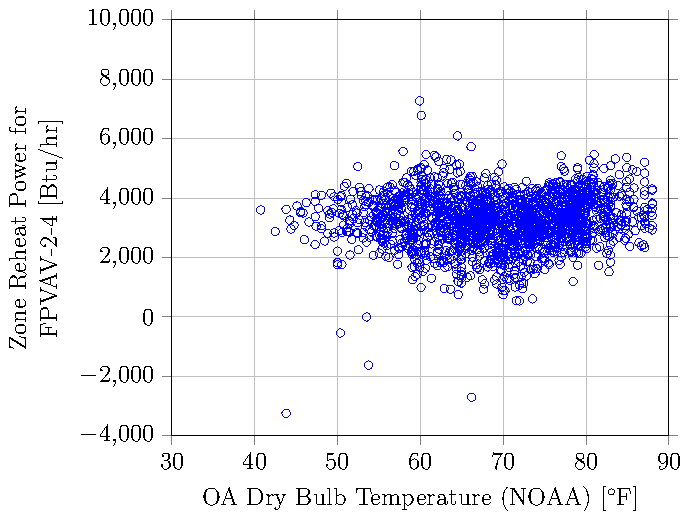
\includegraphics{Plots/2016-10-19-1438-ZoneReheatEnergyforContainerFPVAV24vsOADryBulbTemperatureNOAA.pdf}
\caption{\zoneReheatCaption{2-4}}
\label{fig:2016-10-19-1438-ZoneReheatEnergyforContainerFPVAV24vsOADryBulbTemperatureNOAA}
\end{figure}

% Plots/2016-10-19-1521-ZoneReheatEnergyforContainerFPVAV213vsOADryBulbTemperatureNOAA.tex
\begin{figure}
\centering
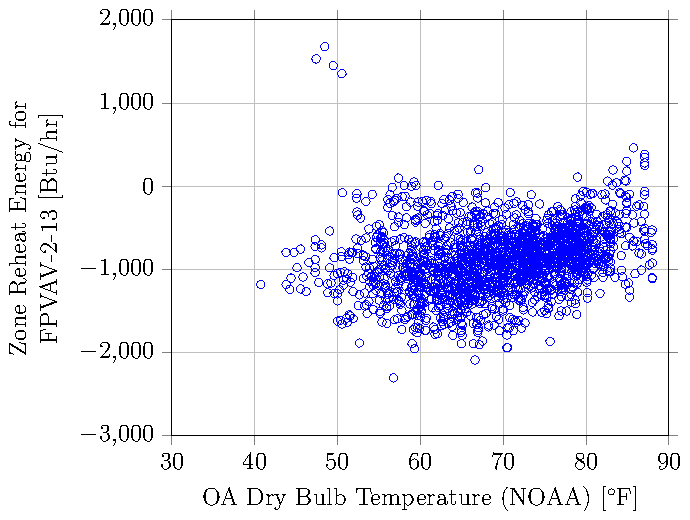
\includegraphics{Plots/2016-10-19-1521-ZoneReheatEnergyforContainerFPVAV213vsOADryBulbTemperatureNOAA.pdf}
\caption{\zoneReheatCaption{2-13}}
\label{fig:2016-10-19-1521-ZoneReheatEnergyforContainerFPVAV213vsOADryBulbTemperatureNOAA}
\end{figure}

Another way to view the accuracy and importance of the plenum           
temperature on the amount of reheat necessary is to look at the         
difference between the discharge temperature and the predicted mixed    
air temperature in the terminal unit under conditions when the reheat   
valve is closed. During these times the values should be nearly equal,  
and the difference should be near zero.                                 

Under the assumption that the plenum temperature is equal to the
corresponding zone temperature, it does not appear as if this assumption
is valid for the corresponding energy calculations. \figref{}
\ref{fig:2017-01-09-1412-TboxDischargeMixedAirTempfromRoomTempforFPVAV27vsTboxPLRforFPVAV27}
shows as much as an \SI{8}{\degreeF} difference for FPVAV-2-7. Because
the value is positive, this means that the plenum temperature is likely
higher than the assumed zone temperature, assuming that the measured
discharge temperature is more accurate that the estimation of the plenum
temperature.                               

\begin{figure}
\centering
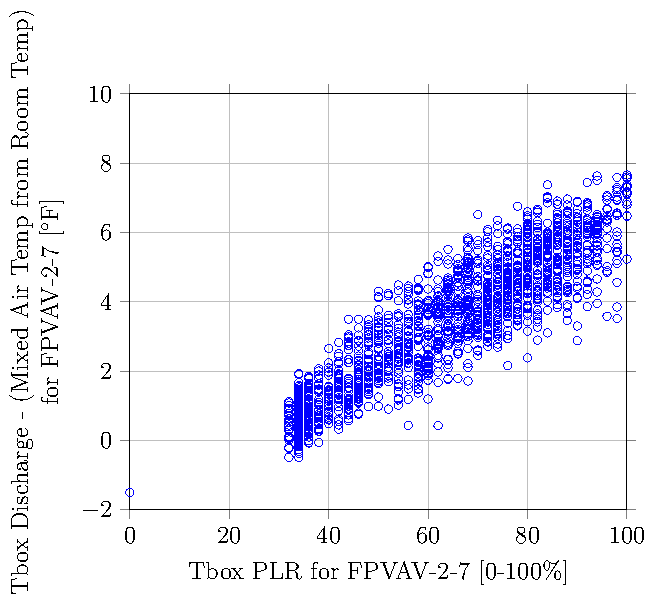
\includegraphics{Plots/2017-01-09-1412-TboxDischargeMixedAirTempfromRoomTempforFPVAV27vsTboxPLRforFPVAV27.pdf}
\caption{Difference between discharge temperature and predicted mixed
air temperature using the zone temperature assumption for FPVAV-2-7.}
\label{fig:2017-01-09-1412-TboxDischargeMixedAirTempfromRoomTempforFPVAV27vsTboxPLRforFPVAV27}
\end{figure}

The opposite case can be seen with FPVAV-2-15, as shown in \figref{}
\ref{fig:2017-01-09-1434-TboxDischargeMixedAirTempfromRoomTempforFPVAV215vsTboxPLRforFPVAV215}.
In this case, the values are all negative, indicating that the plenum
temperature is lower than the zone temperature. The plots are from the
same period and cover a broad range of outdoor air temperatures from
\SI{36}{\degreeF} to \SI{96}{\degreeF}. Both plots do appear linear with
regards to the PLR of the terminal unit. This linearity indicates that there is
some relationship with the plenum temperature and the amount of
conditioned air coming from the parent air handling unit.

\begin{figure}
\centering
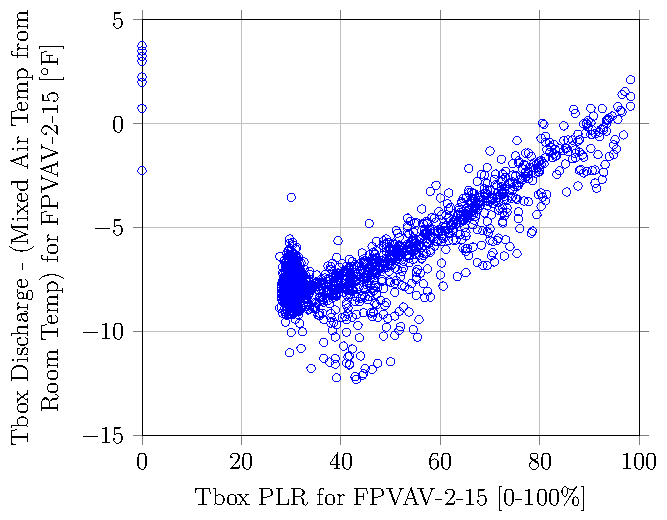
\includegraphics{Plots/2017-01-09-1434-TboxDischargeMixedAirTempfromRoomTempforFPVAV215vsTboxPLRforFPVAV215.pdf}
\caption{Difference between discharge temperature and predicted mixed
air temperature using the zone temperature assumption for TU-2-15.}
\label{fig:2017-01-09-1434-TboxDischargeMixedAirTempfromRoomTempforFPVAV215vsTboxPLRforFPVAV215}
\end{figure}


This linear dependence on the PLR does not carry to all the terminal
units. As a counterexample to the previous plots, FPVAV-2-10 has a
zig-zag pattern. 


\begin{figure}
\centering
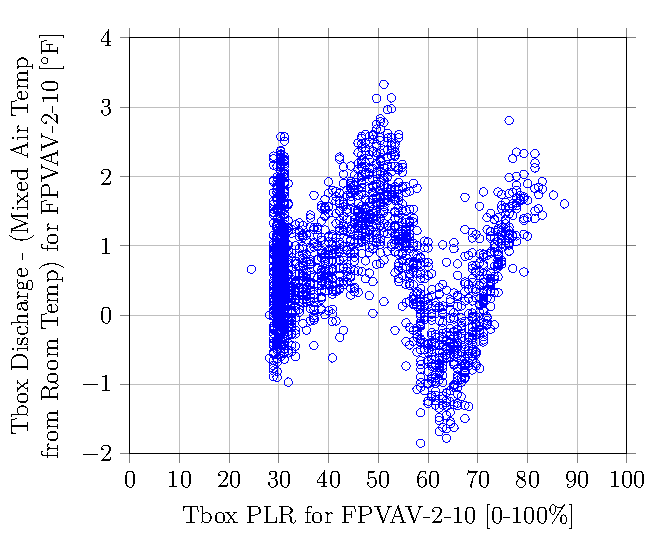
\includegraphics{Plots/2017-01-10-0906-TboxDischargeMixedAirTempfromRoomTempforFPVAV210vsTboxPLRforFPVAV210.pdf}
\caption{Difference between discharge temperature and predicted mixed
air temperature using the zone temperature assumption for FPVAV-2-10.}
\label{fig:2017-01-10-0906-TboxDischargeMixedAirTempfromRoomTempforFPVAV210vsTboxPLRforFPVAV210}
\end{figure}

\section{Analysis of Zone Load Predictions}

An important factor in the optimization methodology is the prediction of
the zone loads at a given time, without access to current live sensor
information. 

Before analyzing how well different zone loads can be predicted, it is
important to gather insight into the nature of the calculated zone load
variable that is proposed to be used as the surrogate for the actual zone load.   

If the zone loads are being met and steady-state conditions are assumed,
the sensible zone load will be
\begin{equation}\label{eq:ApproximateZoneLoad}
    \dot{Q}_{z}=\flow{z} \rhocp{} \left(T_{dis}-T_{z} \right) \approx 1.08 \cdot \flow{z}\left(T_{dis}-T_{z} \right)
\end{equation}
where \(\dot{Q}\) is in units of \si{\btu\per\hour}, \(\flow{z}\) is in CFM, and the temperatures are in \si{\degreeF}.

As a result of the dynamics of how terminal units are                   
controlled in reality, the estimated zone load can vary                 
back and forth, while the true zone load is expected to be              
a smoother function over the course of a day. \figref{}                 
\ref{fig:2016-06-22-1654-ZoneLoadforContainerFPVAV17-TikzData}          
shows how the estimated zone load using \eqreftext{}                    
\ref{eq:ApproximateZoneLoad} can change directionality several times    
over the course of a day. The zone load for terminal unit FPVAV-1-7     
typically varied from 6,000 BTU/hr to 20,000 BTU/hr over the course of  
the week from June 6, 2016, to June 11, 2016.                           

\figref{} \ref{fig:2016-06-22-1643-ZoneLoadforContainerFPVAV22-TikzData}
shows another example of how the estimated zone load may vary throughout
a typical week. \figref{}
\ref{fig:2016-06-22-1643-ZoneLoadforContainerFPVAV22-TikzData} shows the
zone load for FPVAV-2-2, which experiences a significant load compared
to the other terminal units at NCTM. The zone load varies from near
10,000 BTU/hr to near 50,000 BTU/hr at its peak.

With \figref{}
\ref{fig:2016-06-22-1654-ZoneLoadforContainerFPVAV17-TikzData} as
evidence, it is clear that the ``true'' zone load cannot be reasonably
estimated with the trend data that is available in typical BAS systems.
However, the ratio of magnitudes of the load from zone to zone can still
be inferred and be useful in improving the energy efficiency of the
system.  

% Plots/2016-06-22-1654-ZoneLoadforContainerFPVAV17-TikzData.tex
\begin{figure}
\centering
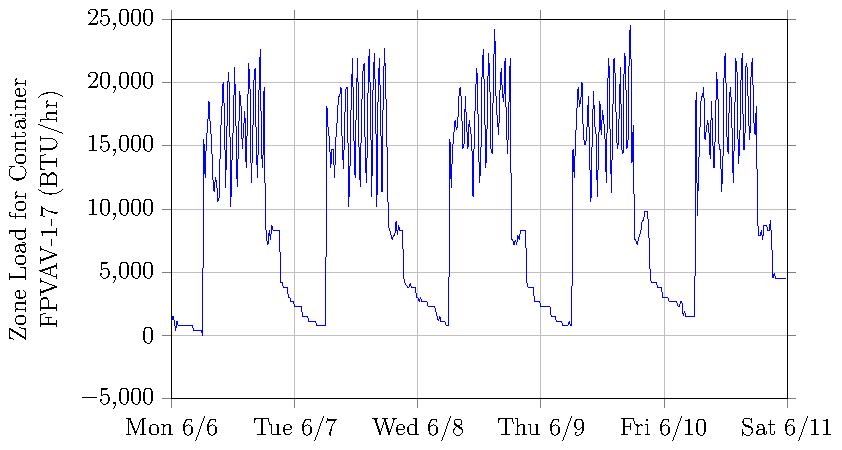
\includegraphics{Plots/2016-06-22-1654-ZoneLoadforContainerFPVAV17-TikzData.pdf}
\caption{Zone load estimation for FPVAV-1-7.}
\label{fig:2016-06-22-1654-ZoneLoadforContainerFPVAV17-TikzData}
\end{figure}

% Plots/2016-06-22-1643-ZoneLoadforContainerFPVAV22-TikzData.tex
\begin{figure}
\centering
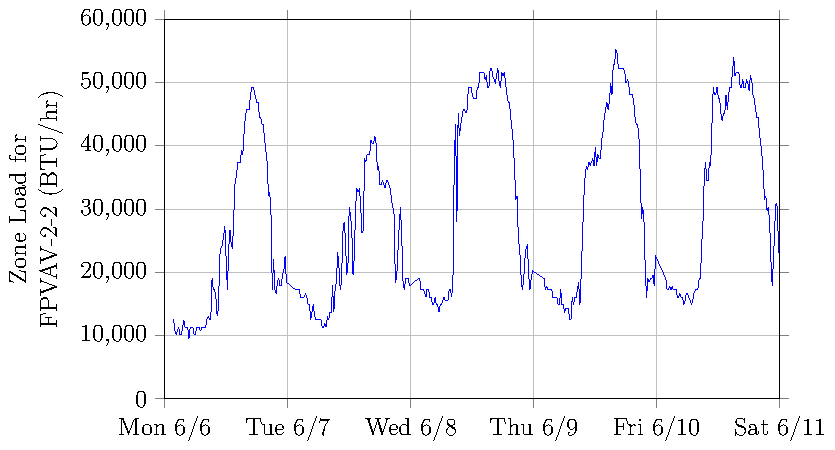
\includegraphics{Plots/2016-06-22-1643-ZoneLoadforContainerFPVAV22-TikzData.pdf}
\caption{Zone load estimation for FPVAV-2-2.}
\label{fig:2016-06-22-1643-ZoneLoadforContainerFPVAV22-TikzData}
\end{figure}



\figref{}
\ref{fig:ZoneLoadforContainerFPVAV214vsOADryBulbTemperatureNOAA} shows
an example of the zone load plotted against outdoor air dry-bulb
temperature. Notice that the load is not a well-defined function of
\(\oat\). This turns out to be the case for many of the internal zones,
which have a higher dependence on the time of day parameters. 

\figref{}
\ref{fig:ZoneLoadforContainerFPVAV29vsOADryBulbTemperatureNOAA} shows
the zone load for FPVAV-2-9 versus \(\oat\). FPVAV-2-9 serves only
internal zones, and the load only ranges from approximately
\SI{0}{\btu\per\hour} to \SI{10000}{\btu\per\hour}.


% Plots/2016-06-22-1704-ZoneLoadforContainerFPVAV214vsOADryBulbTemperatureNOAA.tex
\begin{figure}
\centering
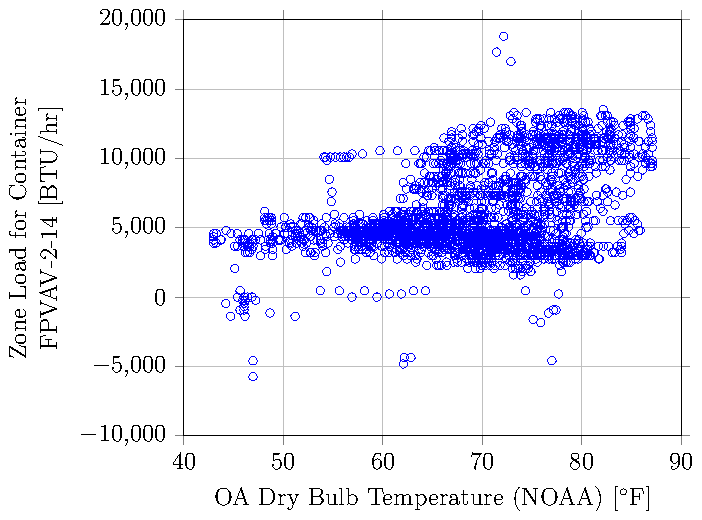
\includegraphics{Plots/2016-06-22-1704-ZoneLoadforContainerFPVAV214vsOADryBulbTemperatureNOAA.pdf}
\caption{Calculated zone load for FPVAV-2-14 during the month of April 2016.}
\label{fig:ZoneLoadforContainerFPVAV214vsOADryBulbTemperatureNOAA}
\end{figure}


\begin{figure}
\centering
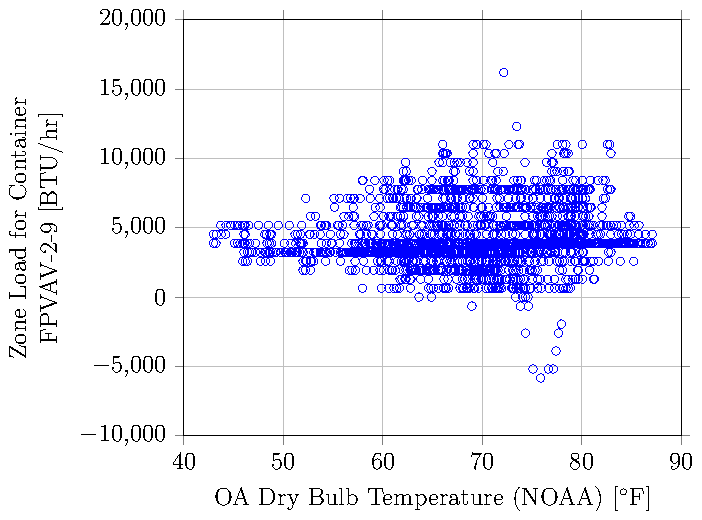
\includegraphics{Plots/2016-06-22-1716-ZoneLoadforContainerFPVAV29vsOADryBulbTemperatureNOAA.pdf}
\caption{Calculated zone load for FPVAV-2-9, which serves only internal space, during the month of April 2016.}
\label{fig:ZoneLoadforContainerFPVAV29vsOADryBulbTemperatureNOAA}
\end{figure}


Statistics related to the predictions of the zone loads for data        
ranging from October 6, 2015, to June 1, 2016, are given in \tableref{} 
\ref{tab:zoneLoadStats}.                                                


%%Data from NCTM Report 2016-06-20 T 12-16.xlsx.
\begin{table}
\centering
\caption{Statistics related to the prediction of the zone loads at NCTM.}
\small
\label{tab:zoneLoadStats}
\begin{tabular}{lrrrr} 
    \toprule
    Terminal Unit & \parbox{2.7cm}{Med. Abs. \\ Error (BTU/hr)} &
    \parbox{2.7cm}{Mean Abs. \\ Error (BTU/hr)} &  \parbox{2cm}{RMSE \\ (BTU/hr)} & \parbox{2cm}{MBE \\ (BTU/hr)} \\
    \midrule
FPVAV-2-7  & 108   & 171   & 298    & -41    \\
FPVAV-2-16 & 135   & 385   & 704    & 59     \\
FPVAV-2-5  & 162   & 221   & 328    & -22    \\
FPVAV-2-12 & 203   & 1,058 & 1,885  & -896   \\
FPVAV-2-6  & 216   & 488   & 836    & 24     \\
FPVAV-2-13 & 270   & 784   & 1,841  & 68     \\
FPVAV-2-10 & 292   & 631   & 1,000  & -87    \\
FPVAV-2-11 & 302   & 708   & 1,062  & -68    \\
FPVAV-2-18 & 324   & 914   & 1,614  & 77     \\
FPVAV-1-11 & 324   & 703   & 1,585  & 115    \\
FPVAV-2-14 & 459   & 1,004 & 1,780  & -9     \\
FPVAV-2-4  & 540   & 1,036 & 2,012  & 84     \\
FPVAV-1-2  & 626   & 1,201 & 2,056  & -385   \\
FPVAV-2-8  & 648   & 991   & 1,519  & -43    \\
FPVAV-2-9  & 648   & 1,236 & 1,763  & 635    \\
FPVAV-2-17 & 691   & 1,386 & 2,327  & 122    \\
FPVAV-2-15 & 756   & 3,852 & 12,353 & 552    \\
FPVAV-1-8  & 945   & 1,371 & 1,978  & 336    \\
FPVAV-2-3  & 972   & 1,789 & 3,587  & -171   \\
FPVAV-2-1  & 1,080 & 1,609 & 2,871  & -559   \\
FPVAV-1-9  & 1,296 & 1,850 & 2,805  & 209    \\
FPVAV-1-5  & 1,404 & 2,463 & 4,105  & -17    \\
FPVAV-1-10 & 1,512 & 2,819 & 4,634  & 1,054  \\
FPVAV-1-1  & 1,598 & 3,783 & 6,267  & -1,359 \\
FPVAV-1-3  & 1,755 & 3,164 & 4,868  & -237   \\
FPVAV-1-6  & 1,814 & 3,186 & 4,861  & 261    \\
FPVAV-1-7  & 2,268 & 2,827 & 3,942  & -326   \\
FPVAV-2-2  & 2,376 & 4,422 & 7,184  & 1,773  \\
FPVAV-1-4  & 3,024 & 5,569 & 8,502  & 19     \\
    \bottomrule
\end{tabular}
\end{table}

The highest errors in the prediction were for FPVAV-1-4, the zone that
has the highest overall zone load in the building, by a significant
margin. It has estimated loads near 50,000 BTU/hr.


%% These items come from the analysis done with plus minus 15 min and 3 degree F OAT bounds in file Batch Plots -- Mitch Dissertation N -- 2016-09-14 0952

An interesting pattern was that the nearest neighbor prediction         
function overpredicted the zone load (as calculated by \eqreftext{}     
\ref{eq:ApproximateZoneLoad}) when the zone cooling load was small or   
was a heating load and underpredicted the zone load during times of     
high cooling load.                                                      

The residual is defined as the predicted value minus the estimated
value, so a positive value indicates overprediction, while a negative
value indicates underprediction.

This bias was seen in every terminal unit in the building, and this bias
occurred with both the largest and smallest terminal units. Figures
\ref{fig:2016-09-14-1028-ZoneLoadResidualforContainerFPVAV22vsZoneLoadforContainerFPVAV22}
through
\ref{fig:2016-09-14-1020-ZoneLoadResidualforContainerFPVAV27vsZoneLoadforContainerFPVAV27}
show examples of this phenomenon. The explanation for this is that the
median of data under similar conditions was used for the prediction. The
function therefore cannot overpredict the highest value or
underpredict the lowest value.  The date period analyzed was from March
1, 2016, to August 1, 2016, ignoring when the AHUs were off, federal
holidays and weekends, and hours from 5 PM to 9 AM. 

\newcommand{\zoneLoadCaption}[1]{Bias in zone load prediction for #1.}


\begin{figure}
\centering
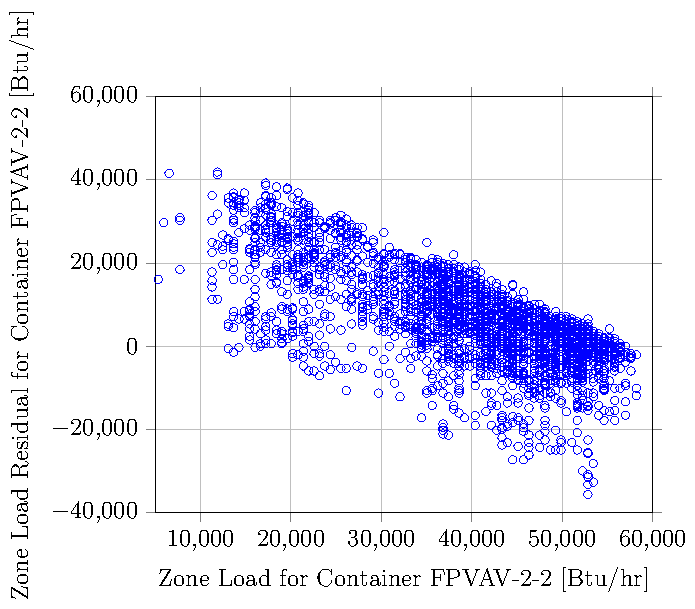
\includegraphics{Plots/2016-09-14-1028-ZoneLoadResidualforContainerFPVAV22vsZoneLoadforContainerFPVAV22.pdf}
\caption{\zoneLoadCaption{FPVAV-2-2}}
\label{fig:2016-09-14-1028-ZoneLoadResidualforContainerFPVAV22vsZoneLoadforContainerFPVAV22}
\end{figure}

% Plots/2016-09-14-1007-ZoneLoadResidualforContainerFPVAV14vsZoneLoadforContainerFPVAV14.tex
\begin{figure}
\centering
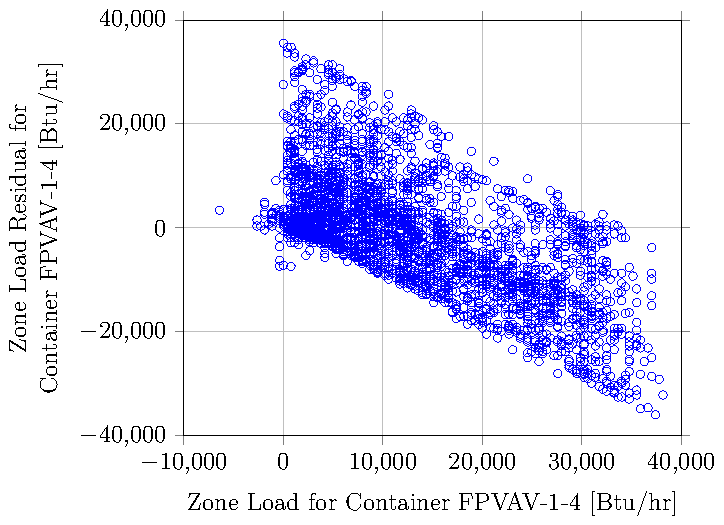
\includegraphics{Plots/2016-09-14-1007-ZoneLoadResidualforContainerFPVAV14vsZoneLoadforContainerFPVAV14.pdf}
\caption{\zoneLoadCaption{FPVAV-1-4}}
\label{fig:2016-09-14-1007-ZoneLoadResidualforContainerFPVAV14vsZoneLoadforContainerFPVAV14}
\end{figure}

% Plots/2016-09-14-1020-ZoneLoadResidualforContainerFPVAV27vsZoneLoadforContainerFPVAV27.tex
\begin{figure}
\centering
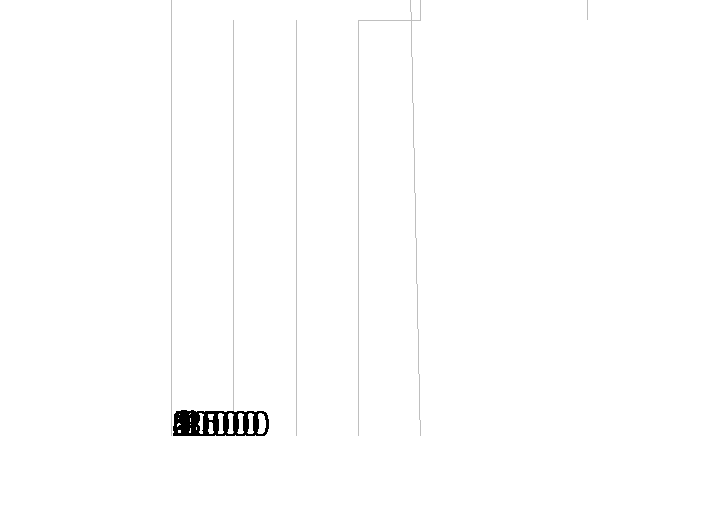
\includegraphics{Plots/2016-09-14-1020-ZoneLoadResidualforContainerFPVAV27vsZoneLoadforContainerFPVAV27.pdf}
\caption{ \zoneLoadCaption{FPVAV-2-7} }
\label{fig:2016-09-14-1020-ZoneLoadResidualforContainerFPVAV27vsZoneLoadforContainerFPVAV27}
\end{figure}


An analysis was also completed regarding the optimal parameters for the 
nearest neighbor approach. The three parameters for the function are    
the time of day threshold, the outdoor air temperature threshold, and   
the number of data points to use.                                       

Three different tests cases for each variable were used. The time of day
threshold was adjusted from 1 timestamp away, 2 timestamps away, and 4
timestamps away. For 15 minute interval data, this means that the
threshold was 15 minutes, 30 minutes, and 1 hour. 

The outdoor air temperature threshold was tested at \SI{1}{\degreeF},
\SI{3}{\degreeF}, and \SI{5}{\degF}. The number of data points used in
the median was 15, 30, and 45. 

The objective function for these tests was the average root mean squared
error (RMSE) divided by the range of the calculated zone loads
for all the terminal units in NCTM, which is defined as CV-RMSE*.

\begin{equation}
    \text{CV-RMSE*} = \frac{\text{RMSE}}{y_{max}-y_{min}}
\end{equation}

Note that for data sets such as zone load which can be both above and
below zero, that the coefficient of variation using the mean as the
normalization factor, a commonly used metric in evaluating model fits,
can be arbitrarily high because the mean can be close to zero (implying
that the zone load is both positive and negative). 

The tests were done for data from January 1\textsuperscript{st}, 2016
through January 1\textsuperscript{st}, 2017. Times when the air handling
units were off and the first and last hour of operation, weekends,  and
federal holidays were all ignored. 

The results show that the goodness-of-fit metrics were insensitive to
the various parameters. In addition, the results indicate that looser
thresholds, which results in more recent data being used, gave the best
model fits. The best average CV-RMSE* was 11.6\% was under the
conditions of thresholds of plus or minus one hour, \SI{5}{\degF}, and
using 45 data points.  The worst models had an average CV-RMSE* of 13.5\%, for
the thresholds of plus or minus 15 minutes, \SI{1}{\degF}, and 45 data
points. The rest of the tests are also shown in \tableref{}
\ref{tab:ZoneLoadTestingResults}.

A main takeaway of the tests, however, was that the results were        
insensitive to the parameters. This means that the parameters may be    
adjusted for benefits in other areas such as performance. By having     
large thresholds and requiring less data points, less historical data   
needs to be searched, and the time to complete the calculations is      
reduced.                                                                

A plot of these results in order of predictive ability is shown in
\figref{} \ref{fig:ZoneLoadInOrder}. 


\begin{table}
\centering
\caption{Testing results for zone load prediction.}
\label{tab:ZoneLoadTestingResults}
\begin{tabular}{@{}lllcS[table-format=2.2,round-mode=off]@{}}
\toprule
Run & TS & \(T_{oa} \) & \# of Data Points & {Average \(\left(\frac{\text{RMSE}}{\heatenergy{z,max}-\heatenergy{z,min}}\right)\) (\%)} \\ \midrule
1   & 1  & 1           & 15                & 10.12          \\
2   & 2  & 1           & 15                & 9.68           \\
3   & 4  & 1           & 15                & 9.80           \\
4   & 1  & 3           & 15                & 9.61           \\
5   & 2  & 3           & 15                & 9.41           \\
6   & 4  & 3           & 15                & 8.97           \\
7   & 1  & 5           & 15                & 9.28           \\
8   & 2  & 5           & 15                & 9.18           \\
9   & 4  & 5           & 15                & 8.98           \\
10  & 1  & 1           & 30                & 10.58          \\
11  & 2  & 1           & 30                & 10.07          \\
12  & 4  & 1           & 30                & 9.39           \\
13  & 1  & 3           & 30                & 9.95           \\
14  & 2  & 3           & 30                & 9.63           \\
15  & 4  & 3           & 30                & 9.16           \\
16  & 1  & 5           & 30                & 9.61           \\
17  & 2  & 5           & 30                & 9.25           \\
18  & 4  & 5           & 30                & 9.00           \\
19  & 1  & 1           & 45                & 10.75          \\
20  & 2  & 1           & 45                & 10.47          \\
21  & 4  & 1           & 45                & 9.80           \\
22  & 1  & 3           & 45                & 10.08          \\
23  & 2  & 3           & 45                & 9.58           \\
24  & 4  & 3           & 45                & 9.32           \\
25  & 1  & 5           & 45                & 9.74           \\
26  & 2  & 5           & 45                & 9.52           \\
27  & 4  & 5           & 45                & 9.08           \\ \bottomrule
\end{tabular}
\end{table}


% Plots/02/2017-06-09-ZoneLoadPredOrder.tex
\begin{figure}
\centering

\includegraphics{Plots/02/2017-06-09-ZoneLoadPredOrder.pdf}
\caption{Zone load prediction results using the Nearest Neighbor approach.}
\label{fig:ZoneLoadInOrder}
\end{figure}



% \section{Analysis of the Zone Temperature Prediction} 
% 
% The same prediction algorithm for the zone load can be used for
% predicting the zone temperatures. The zone temperatures will be a
% function of the time of day, day of week, and the outdoor air
% temperature. 


% \section{Analysis of the Mixed Air Temperature in Series Terminal Unit and Reheat Assumption}


\section{Analysis of the Critical Zones}

The critical zone/damper could be used to determine the static pressure 
setpoint that can be used to supply the desired flows found from the    
optimization. An important consideration in the methodology is checking 
how well this assumption holds. Data from NCTM was used to test the     
validity of the approach.                                               

The following figures show the maximum damper position of the terminal  
units for each of the air handlers during the month of April 2016.      
During this time, for AHU-2-1 and AHU-2-2, there was no time in which   
a terminal unit damper was fully open, which indicates that there is    
potential for the supply air static pressure setpoints of these AHUs to 
be reduced.                                                             

\newcommand{\MaxDampCaption}[1]{Maximum damper position of all terminal units versus \(\oat{}\) for #1 during the month of April 2016.}

\begin{figure}
\centering
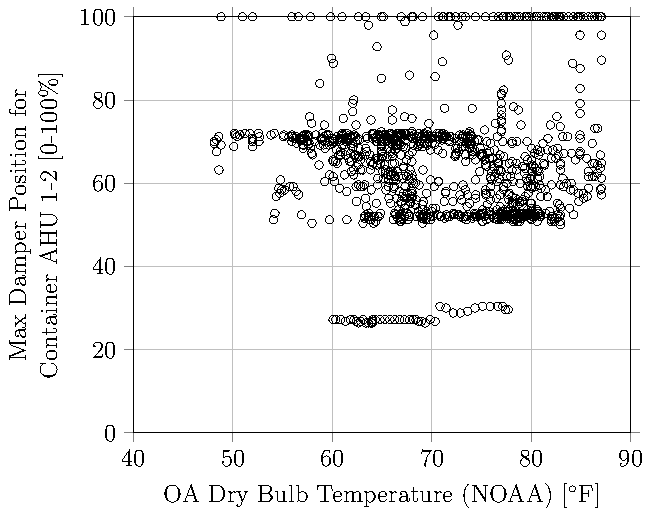
\includegraphics{Plots/MaximumDamperPosition-1-2.pdf} 
\caption{\MaxDampCaption{AHU-1-2}}
\label{fig:MaxDamperPositionforContainerAHU12vsOADryBulbTemperatureNOAA}
\end{figure}

\begin{figure}
\centering
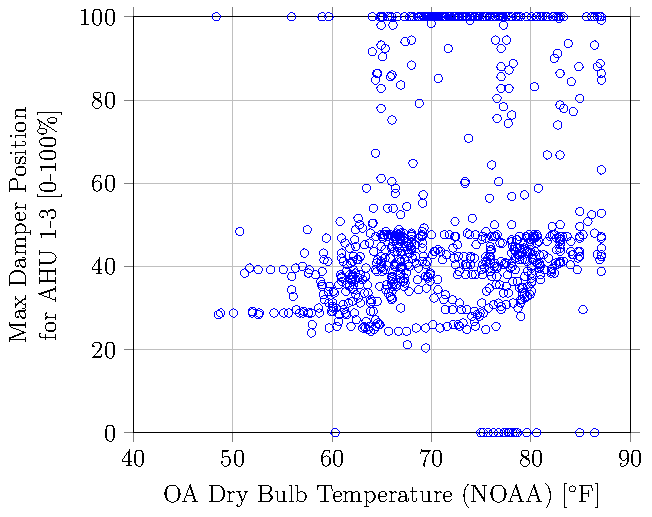
\includegraphics{Plots/MaximumDamperPosition-1-3.pdf}
\caption{\MaxDampCaption{AHU-1-3}}
\label{fig:MaxDamperPositionforContainerAHU13vsOADryBulbTemperatureNOAA}
\end{figure}


\begin{figure}
\centering
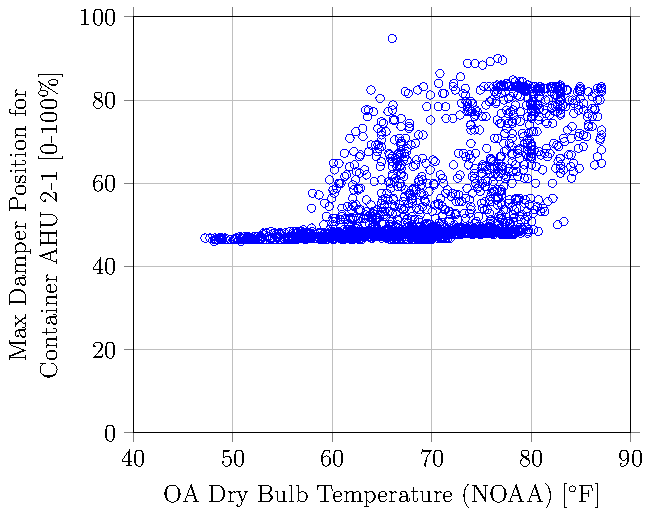
\includegraphics{Plots/MaximumDamperPosition-2-1.pdf}
\caption{\MaxDampCaption{AHU-2-1}}
\label{fig:MaxDamperPositionforContainerAHU21vsOADryBulbTemperatureNOAA}
\end{figure}

\begin{figure}
\centering
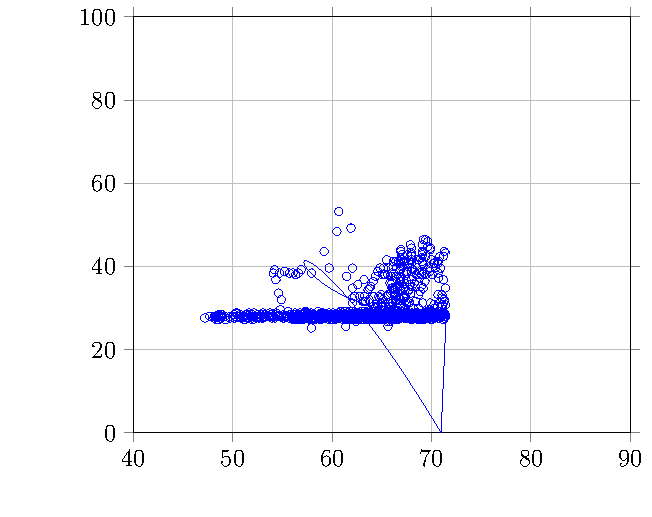
\includegraphics{Plots/2016-06-06-1427-MaxDamperPositionforContainerAHU22vsOADryBulbTemperatureNOAA.pdf}
\caption{\MaxDampCaption{AHU-2-2}}
\label{fig:MaxDamperPositionforContainerAHU22vsOADryBulbTemperatureNOAA}
\end{figure}

\begin{figure}
\centering
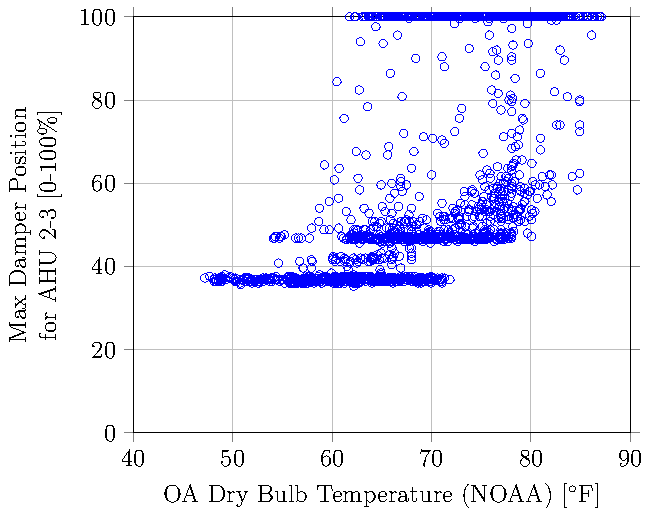
\includegraphics{Plots/2016-06-06-1454-MaxDamperPositionforContainerAHU23vsOADryBulbTemperatureNOAA.pdf}
\caption{\MaxDampCaption{AHU-2-3}}
\label{fig:MaxDamperPositionforContainerAHU23vsOADryBulbTemperatureNOAA}
\end{figure}

An investigation into the critical zones based on historical data was
completed. 15 minute interval data from January 1, 2016, through June 1,
2016, was used to check which damper positions were most open at a given
timestamp. \tableref{} \ref{tab:AHU12CriticalZone} shows the results of
this analysis. In all five of the applicable air handling units, there
is a damper that is critical at least 59\% of the time. 

%% Comes from file 2016-06-08-1603-CriticalZoneAnalysis.xlsx
%% Run from 2016-01-01 to 2016-06-01.
%% Assumes that the AHU is on. 
\begin{table}
\centering
\caption{Percentage of time that different terminal units for various AHUs were the most open during the period of January 1, 2016 - June 1, 2016.}
\label{tab:AHU12CriticalZone}
\begin{tabular}{@{}clS[table-format=5.0,round-mode=off]S[table-format=2.0]@{}}
\toprule
AHU (\# of term. units)      & Unit       & {Count of Max} & {Percent as Critical (\%)} \\ \midrule
\multirow{3}{*}{AHU-1-2 (4)} & FPVAV-1-8  & 3518           & 68                         \\
                             & FPVAV-1-9  & 1281           & 25                         \\
                             & 2 others   & 354            & 7                          \\ \midrule
\multirow{3}{*}{AHU-1-3 (6)} & FPVAV-1-5  & 2331           & 59                         \\
                             & FPVAV-1-4  & 1006           & 25                         \\
                             & 4 others   & 622            & 15                         \\ \midrule
\multirow{3}{*}{AHU-2-1 (3)} & FPVAV-2-1  & 10965          & 79                         \\
                             & FPVAV-2-2  & 2648           & 19                         \\
                             & FPVAV-2-3  & 258            & 2                          \\ \midrule
\multirow{3}{*}{AHU-2-2 (8)} & FPVAV-2-18 & 10003          & 72                         \\
                             & FPVAV-2-14 & 3171           & 23                         \\
                             & 6 others   & 648            & 5                          \\ \midrule
\multirow{3}{*}{AHU-2-3 (7)} & FPVAV-2-6  & 9883           & 72                         \\
                             & FPVAV-2-11 & 3743           & 27                         \\
                             & FPVAV-2-10 & 184            & 1                          \\ \midrule
\end{tabular}
\end{table}

This analysis was not actively used to optimize the air handling        
unit system at NCTM. However, if more information were available        
regarding the fan and duct system, it could be used to also optimize    
the supply air static pressure setpoint in combination with the supply  
air temperature. It is useful to see, however, that potential exists    
to reduce fan power and the pressure drop throughout the system, which  
would aid in the goal of energy efficient operation.                    

\section{Accuracy of Mechanical Specifications}

In the simplified analysis and modeling being proposed, it would be     
ideal if the specifications in the mechanical drawings can be used      
directly. One important parameter is the design flow rate for the       
terminal unit. \tableref{} \ref{tab:TerminalUnitInformation} shows      
the design flow rates for all the series fan powered terminal units     
in the NCTM building. The results show that the design specifications   
were sufficiently accurate. All data that were available at the time    
(October 6, 2015, through June 7, 2016) were analyzed to capture        
a large number of timestamps (over 22,000 timestamps). Over half        
the absolute differences between the measured maximum flow and the      
specified design flow are less than \SI{100}{\cfm}. There are several   
reasons for potential differences between the maximum measured flow and 
the design flow rates in the mechanical drawings. It may be the case    
that the terminal unit was oversized and the design flow rate was never 
necessary. There may be bias in the flow rate measurements.             

The largest percent difference and absolute difference between the
measured maximum flow rate and design value was for FPVAV-1-9. The
difference was due to less than 15 outliers in the data (out of over
20,000 data points in total), and if they were to be removed, the
maximum is in line with the design value of 1,200 CFM for the vast
majority of the data, as seen in \figref{}
\ref{fig:FPVAV19AIRVOLUMEvsFPVAV19DMPRCOMD}. 

%%See file: Batch Plots -- Mitch Dissertation N -- 2016-06-09 0942.xlsx
\begin{table}
\centering
\footnotesize
\caption{Comparison of design flow specifications to actual data.}
\label{tab:TerminalUnitDesignSpecCheck}
\begin{tabular}{@{}llS[table-format=4.0,round-mode=off]S[table-format=4.0,round-mode=off]S[round-mode=off]@{}}
\toprule
AHU         & Terminal Unit & { \parbox{1.5cm}{\centering  Flow\\(CFM)} } & { \parbox{2.7cm}{Maximum Meas. \\  Flow (CFM)} } & { \parbox{1.5cm}{Difference \\ (CFM)} } \\ \midrule
AHU-1-2     & FPVAV-1-7     & 1400                                        & 1496                                             & 96                                      \\ \cmidrule(r){2-5}
(5 hp)      & FPVAV-1-8     & 700                                         & 840                                              & 140                                     \\ \cmidrule(r){2-5}
            & FPVAV-1-9     & 1200                                        & 1688                                             & 488                                     \\ \cmidrule(r){2-5}
            & FPVAV-1-10    & 1600                                        & 1712                                             & 112                                     \\ \midrule
AHU-1-3     & FPVAV-1-1     & 1480                                        & 1676                                             & 196                                     \\ \cmidrule(r){2-5}
(7.5 hp)    & FPVAV-1-2     & 1160                                        & 1240                                             & 80                                      \\ \cmidrule(r){2-5}
            & FPVAV-1-3     & 1300                                        & 1364                                             & 64                                      \\ \cmidrule(r){2-5}
            & FPVAV-1-4     & 1400                                        & 1760                                             & 360                                     \\ \cmidrule(r){2-5}
            & FPVAV-1-5     & 1040                                        & 612                                              & -428                                    \\ \cmidrule(r){2-5}
            & FPVAV-1-6     & 1120                                        & 1288                                             & 168                                     \\ \midrule
AHU-2-1     & FPVAV-2-1     & 2000                                        & 2016                                             & 16                                      \\ \cmidrule(r){2-5}
(7.5 hp)    & FPVAV-2-2     & 2200                                        & 2060                                             & -140                                    \\ \cmidrule(r){2-5}
            & FPVAV-2-3     & 1800                                        & 1824                                             & 24                                      \\ \midrule
AHU-2-2     & FPVAV-2-9     & 2400                                        & 2448                                             & 48                                      \\ \cmidrule(r){2-5}
(10 hp)     & FPVAV-2-12    & 500                                         & 452                                              & -48                                     \\ \cmidrule(r){2-5}
            & FPVAV-2-13    & 1000                                        & 1032                                             & 32                                      \\ \cmidrule(r){2-5}
            & FPVAV-2-14    & 850                                         & 892                                              & 42                                      \\ \cmidrule(r){2-5}
            & FPVAV-2-15    & 1400                                        & 1332                                             & -68                                     \\ \cmidrule(r){2-5}
            & FPVAV-2-16    & 500                                         & 484                                              & -16                                     \\ \cmidrule(r){2-5}
            & FPVAV-2-17    & 1280                                        & 1304                                             & 24                                      \\ \cmidrule(r){2-5}
            & FPVAV-2-18    & 600                                         & 604                                              & 4                                       \\ \midrule
AHU-2-3     & FPVAV-2-4     & 2000                                        & 1944                                             & -56                                     \\ \cmidrule(r){2-5}
(7.5 hp)    & FPVAV-2-5     & 600                                         & 504                                              & -96                                     \\ \cmidrule(r){2-5}
            & FPVAV-2-6     & 400                                         & 228                                              & -172                                    \\ \cmidrule(r){2-5}
            & FPVAV-2-7     & 200                                         & 252                                              & 52                                      \\ \cmidrule(r){2-5}
            & FPVAV-2-8     & 1200                                        & 1184                                             & -16                                     \\ \cmidrule(r){2-5}
            & FPVAV-2-10    & 540                                         & 588                                              & 48                                      \\ \cmidrule(r){2-5}
            & FPVAV-2-11    & 560                                         & 656                                              & 96                                      \\ \bottomrule
\end{tabular}
\end{table}

%%See file: Batch Plots -- Mitch Dissertation N -- 2016-06-09 0942.xlsx
\begin{figure}
\centering
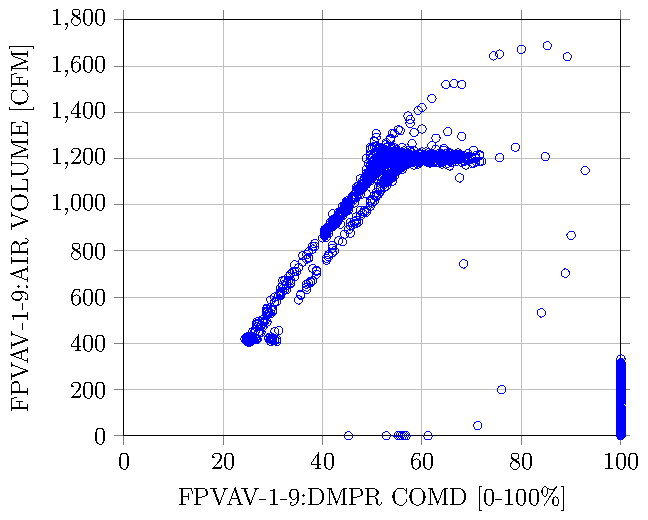
\includegraphics{Plots/2016-06-09-1038-FPVAV19AIRVOLUMEvsFPVAV19DMPRCOMD.pdf}
\caption{Damper position versus primary air flow for FPVAV-1-9.}
\label{fig:FPVAV19AIRVOLUMEvsFPVAV19DMPRCOMD}
\end{figure}


\section{Optimal Supply Air Temperature Results}\label{sec:OptimalSupplyAirTemperatureResults}

The methods described in the previous sections were used to determine
the optimal supply air temperature for various air handling units at the
NCTM building.  \figref{}
\ref{fig:2016-11-30-1004-AHU23MixedAirTemp-TikzData} shows the results
for AHU-2-3 during the work week from Monday, November 7, 2016, through
Friday, November 11, 2016.  During that week, the actual \(\sat\) hovered
between \SI{58}{\degreeF} and \SI{60}{\degreeF}. The optimal \(\sat\) was predicted using
different parameters for the simple fan curve exponent and plenum
temperature.  The optimization was completed using a fan exponent of 2
and 3, and the plenum temperature was assumed to be the room temperature
or assumed to be the static median values shown in \tableref{}
\ref{tab:plenumStatistics}.  Notice that even with the fan curve
exponent varying from 2 to 3, the optimal \(\sat\) is approximately
66\(^\circ\)F, 7\(^\circ\)F higher than the current operation. 

It is also apparent that for this case study that the optimal supply air
temperature is near the maximum of the search range.  The maximum
possible \(\sat\) searched is the minimum between the \(\mat\) and the
minimum calculated discharge temperature. The \(\sat\) cannot be above
the \(\mat\) because that would require heating in the air handling
unit, and cannot be above the minimum calculated discharge temperature
because then that particular zone would be starved for cooling capacity.
For the second floor air handling units, the minimum discharge
temperature is always less than the mixed air temperature indicating
that cooling will always be required.  

\figref{} \ref{fig:2016-11-30-0943-AHU21MixedAirTemp-TikzData} shows the
results for the same computations as \figref{}
\ref{fig:2016-11-30-1004-AHU23MixedAirTemp-TikzData}, but for AHU-2-1.
AHU-2-1 has 3 terminal units supporting a computer lab with higher
measured loads than the rest of the second floor.  The \(\mat\) is also
shown in \figref{} \ref{fig:2016-11-30-0943-AHU21MixedAirTemp-TikzData}
for reference. The optimal \(\sat\) appears to be higher than the
current operation, although a smaller difference compared to AHU-2-3
shown in \figref{} \ref{fig:2016-11-30-1004-AHU23MixedAirTemp-TikzData}.


\figref{} \ref{fig:2016-11-16-1636-AHU22MixedAirTemp-TikzData} shows the
results for AHU-2-2.  In this case, the actual operation is near the
estimated optimal \(\sat\).

\begin{figure}
\centering
\includegraphics{Plots/2016-11-30-1004-AHU23MixedAirTemp-TikzData.pdf}
\caption{Optimal supply air temperature for AHU-2-3.}
\label{fig:2016-11-30-1004-AHU23MixedAirTemp-TikzData}
\end{figure}

\begin{figure}
\centering
\includegraphics{Plots/2016-11-30-0943-AHU21MixedAirTemp-TikzData.pdf}
\caption{Optimal supply air temperature for AHU-2-1.}
\label{fig:2016-11-30-0943-AHU21MixedAirTemp-TikzData}
\end{figure}

\begin{figure}
\centering
\includegraphics{Plots/2016-11-16-1636-AHU22MixedAirTemp-TikzData.pdf}
\caption{Optimal supply air temperature for AHU-2-2.}
\label{fig:2016-11-16-1636-AHU22MixedAirTemp-TikzData}
\end{figure}

\section{Savings Potential}

The potential for energy savings at the NCTM building was investigated
for the second floor AHUs. 

Energy savings were estimated for a period from June
1\textsuperscript{st}, 2016 to January 1\textsuperscript{st}, 2017.
Weekends, times when the AHUs were off, federal holidays, and times from
5:00 PM to 9:00 AM were all ignored. 

Also, since the calculation of reheat power in the terminal units had   
a high uncertainty level, it was decided to ignore times in which at    
least one of the reheat valves in the terminal units was open. Because  
most of the necessary reheat can be accomplished by mixing plenum air   
in the series fan powered terminal units, this only removed a small     
portion of the data. In this sense, the only components to the AHU      
energy were the cooling energy at the cooling coil and the fan energy.  

To provide a sense of the sensitivity to the assumed parameters in the
optimization, savings were determined using different exponents ranging
from 2 to 3 for the PLR curve, along with the plenum temperature assumed
to be the corresponding room temperature and the estimated constant
plenum temperatures shown in \tableref{} \ref{tab:plenumStatistics}. 

Based on the optimal supply air temperatures shown in Section
\ref{sec:OptimalSupplyAirTemperatureResults}, the potential savings in
AHU-2-1 and AHU-2-2 was small since the systems are already
operating near optimal. However, the savings potential in AHU-2-3
appeared promising since there was approximately a \SI{5}{\degreeF}
difference between the operating supply air temperature and the
predicted optimal supply air temperature. The savings results for
AHU-2-3 under various different assumptions is shown in \tableref{}
\ref{tab:NCTMAHU23SavingsResults}.

\figref{}
\ref{fig:2017-01-24-1607-VariableTotalPowervsOADryBulbTemperatureNOAA}
shows the difference in the combined energy of the fan and cooling from
actual to optimal. Periods in which reheat was occurring were ignored
in the analysis. As expected, the energy use has a dependence on
\(\oat\) and the optimal is less than the actual at all times.
Regardless of the different parameters tested, over 20\% savings were
found for AHU-2-3.


%The optimal profile has a 3-Parameter cooling shape, as
%described in \cite{ASHRAE2014}. 

The energy savings were primarily caused by increasing the supply air
temperature, as seen in \figref{}
\ref{fig:2017-01-25-1121-VariableSupplyAirTempvsOADryBulbTemperatureNOAA}.
There already was a supply air temperature reset programmed for AHU-2-3,
but the optimal reset would, in general, have a higher \(\sat\). 


\begin{figure}
\centering
\includegraphics{Plots/2017-01-24-1607-VariableTotalPowervsOADryBulbTemperatureNOAA.pdf}
\caption{Energy savings for AHU-2-3 assuming a fan PLR exponent of 2 and
plenum temperatures equal to the corresponding room temperature. There
is a 13.98 MMBTU difference, or 26\%.}
\label{fig:2017-01-24-1607-VariableTotalPowervsOADryBulbTemperatureNOAA}
\end{figure}

%  Plots/2017-01-25-1121-VariableSupplyAirTempvsOADryBulbTemperatureNOAA.tex
\begin{figure}
\centering
\includegraphics{Plots/2017-01-25-1121-VariableSupplyAirTempvsOADryBulbTemperatureNOAA.pdf}
\caption{Supply air temperature difference between actual and optimal
for AHU-2-3.}
\label{fig:2017-01-25-1121-VariableSupplyAirTempvsOADryBulbTemperatureNOAA}
\end{figure}

% Table generated by Excel2LaTeX from sheet 'Sheet1'
% This comes from files located with filenames like:
% 2017-01-18 11-06 AHU-2-3 No Reheat 6-1through1-1-RoomTemps.xlsx

%Project:	Mitch Dissertation NCTM	
%Scope:	NCTM/2ndFloorAHUs/AHU 2-3	
%Y Axis Parameters:	Fan plus Cooling Energy AHU Actual - Exponent 2 for AHU 2-3	Y Axis 1
	%Variable-TotalPower	Y Axis 2
%Date Period:	6/1/2016 - 1/1/2017	
%Time Alignment Interval	15 minutes	
%Ignoring:	When AHU is Off	
	%Sundays	
	%Saturdays	
	%Federal Holidays	
	%Hours from 17:00 to 9:00	
	%When Sum of FPVAV Valve Positions for AHU 2-3 is greater than 1	



\begin{table}
  \centering
  \caption{Savings results for AHU-2-3, depending on model assumptions.}
  \begin{tabular}{C{2cm}C{4cm}R{2cm}R{2cm}r}
        \toprule
        Fan Exponent & Plenum Temperature Assumption & Actual (MMBTU) & Savings (MMBTU) & \% Savings \\
    \midrule
    2 & Room Temperatures  & 53.43 & 13.98 & 26\% \\
    3 & Room Temperatures  & 51.46 & 12.01 & 23\% \\
    2 & Static Temperature & 53.71 & 15.51 & 29\% \\
    3 & Static Temperature & 51.73 & 13.53 & 26\% \\
\bottomrule
    \end{tabular}%
  \label{tab:NCTMAHU23SavingsResults}%
\end{table}%


\section{Discussion}

A first comment is that it appears plausible that the ``zone load''     
can be reasonably estimated to provide useful information with regards  
to optimization. In fact, the general relationship in the size of the   
thermal loads of the different zones is more important than the precise 
value, which is difficult to estimate.        

The second is that the design specifications from mechanical drawings
can be used as the first approximation for flows and power.  There was
general agreement between the terminal unit design flows and the actual
maximum realized flows at NCTM, as seen in \tableref{}
\ref{tab:TerminalUnitDesignSpecCheck}. 

A third conclusion is that the uncertainty in the optimal \(\sat\)      
was small enough that in most cases the current operation at NCTM       
does not fall within the bounds. In the cases shown in \figref{}        
\ref{fig:2016-11-30-1004-AHU23MixedAirTemp-TikzData} through \figref{}  
\ref{fig:2016-11-16-1636-AHU22MixedAirTemp-TikzData}, the optimal       
\(\sat\) was higher than the current operation.                         

